\section{Benchmark Results}
\label{sec:experiment}
This section presents the evaluation of Rex-Omni across multiple visual perception tasks, such as common, long-tailed, and dense object detection, referring object detection, and object pointing. For each task, we outline the benchmark datasets, experimental settings, and evaluation metrics.

\subsection{Common Object Detection}
\label{sec:coco}
Common object detection refers to the task of detecting objects from a predefined set of categories that frequently appear in real-world scenarios. The goal of this task is to evaluate the model's baisc ability to accurately identify and localize these common objects.

\begin{table*}[t]
    \centering
    \resizebox{1.0\textwidth}{!}{
    \begin{tabular}{cc|cc|cccccccccc}
\toprule
\multirow{2}{*}{Type} & \multirow{2}{*}{Method} & \multirow{2}{*}{Zero-Shot} & \multirow{2}{*}{\begin{tabular}[c]{@{}c@{}}Score \\ Thresh.\end{tabular}} & \multicolumn{10}{c}{COCO} \\
\cline{5-14}
 &  &  &  & \multicolumn{1}{c|}{mAP} & \begin{tabular}[c]{@{}c@{}}R@IoU\\ 0.5\end{tabular} & \begin{tabular}[c]{@{}c@{}}P@IoU\\ 0.5\end{tabular} & \multicolumn{1}{c|}{\begin{tabular}[c]{@{}c@{}}F1@IoU\\ 0.5\end{tabular}} & \begin{tabular}[c]{@{}c@{}}R@IoU\\ 0.95\end{tabular} & \begin{tabular}[c]{@{}c@{}}P@IoU\\ 0.95\end{tabular} & \multicolumn{1}{c|}{\begin{tabular}[c]{@{}c@{}}F1@IoU\\ 0.95\end{tabular}} & \begin{tabular}[c]{@{}c@{}}R@\\ mIoU\end{tabular} & \begin{tabular}[c]{@{}c@{}}P@\\ mIoU\end{tabular} & \begin{tabular}[c]{@{}c@{}}F1@\\ mIoU\end{tabular} \\
\midrule
\multirow{7}{*}{Closed-set}
& Faster RCNN-R50          & No  & 0.42 & \multicolumn{1}{c|}{38.4} & 60.4 & 60.7 & \multicolumn{1}{c|}{60.6} & 4.9  & 12.6 & \multicolumn{1}{c|}{7.1}  & 43.2 & 54.2 & 48.1 \\
& DETR-R50                 & No  & 0.78 & \multicolumn{1}{c|}{41.5} & 59.6 & 73.9 & \multicolumn{1}{c|}{65.9} & 10.6 & 19.0 & \multicolumn{1}{c|}{13.6} & 42.9 & 55.3 & 48.3 \\
& DyHead-R50               & No  & 0.24 & \multicolumn{1}{c|}{45.9} & 58.1 & 76.6 & \multicolumn{1}{c|}{66.1} & 11.9 & 20.6 & \multicolumn{1}{c|}{15.0} & 44.8 & 60.1 & 51.3 \\
& DAB-DETR-R50             & No  & 0.31 & \multicolumn{1}{c|}{44.4} & 59.2 & 77.4 & \multicolumn{1}{c|}{67.1} & 10.5 & 18.5 & \multicolumn{1}{c|}{13.4} & 43.8 & 58.8 & 50.2 \\
& Deformable-DETR-R50      & No  & 0.34 & \multicolumn{1}{c|}{49.4} & 62.6 & 78.5 & \multicolumn{1}{c|}{69.7} & 14.8 & 17.7 & \multicolumn{1}{c|}{17.7} & 48.7 & 62.4 & 54.7 \\
& DINO-R50                 & No  & 0.30 & \multicolumn{1}{c|}{51.7} & 62.6 & 76.5 & \multicolumn{1}{c|}{68.8} & 17.8 & 25.8 & \multicolumn{1}{c|}{21.1} & 50.0 & 62.4 & 55.6 \\
& DINO-Swin-L              & No  & 0.32 & \multicolumn{1}{c|}{59.6} & \textbf{69.8} & \textbf{82.5} & \multicolumn{1}{c|}{\textbf{75.6}} & \textbf{22.2} & \textbf{29.7} & \multicolumn{1}{c|}{\textbf{25.4}} & \textbf{57.0} & \textbf{68.2} & \textbf{62.1} \\
\midrule
Open-set & Grounding DINO-Swin-T & Yes & 0.37 & \multicolumn{1}{c|}{51.5} & 62.8 & 78.4 & \multicolumn{1}{c|}{69.8} & 20.5 & 26.2 & \multicolumn{1}{c|}{23.0} & 54.6 & 58.8 & 56.6 \\
\midrule
\multirow{10}{*}{MLLM}
& DeepSeek-VL2-Tiny         & UNK & - & \multicolumn{1}{c|}{-} & 29.4 & 55.0 & \multicolumn{1}{c|}{38.2} & 5.9  & 13.0 & \multicolumn{1}{c|}{8.1}  & 20.0 & 38.6 & 26.3 \\
& OVIS2.5-9B                & UNK & - & \multicolumn{1}{c|}{-} & 60.0 & 45.3 & \multicolumn{1}{c|}{51.6} & 8.4  & 8.0  & \multicolumn{1}{c|}{8.2}  & 39.3 & 31.0 & 34.6 \\
& Mimo-VL-7B                & UNK & - & \multicolumn{1}{c|}{-} & 56.2 & 56.9 & \multicolumn{1}{c|}{56.5} & 6.1  & 7.4  & \multicolumn{1}{c|}{6.7}  & 35.3 & 36.4 & 35.9 \\
& OVIS2.5-2B                & UNK & - & \multicolumn{1}{c|}{-} & 63.1 & 50.7 & \multicolumn{1}{c|}{56.2} & 10.4 & 10.1 & \multicolumn{1}{c|}{10.3} & 42.6 & 35.4 & 38.7 \\
& DeepSeek-VL2-Small        & UNK & - & \multicolumn{1}{c|}{-} & 52.1 & 73.3 & \multicolumn{1}{c|}{60.9} & 12.5 & \textbf{18.5} & \multicolumn{1}{c|}{14.9} & 39.1 & 55.4 & 45.9 \\
& Qwen2.5-VL-7B             & UNK & - & \multicolumn{1}{c|}{-} & 55.4 & 75.8 & \multicolumn{1}{c|}{64.0} & 10.6 & 15.5 & \multicolumn{1}{c|}{12.6} & 39.5 & 54.2 & 45.7 \\
& Qwen2.5-VL-3B             & UNK & - & \multicolumn{1}{c|}{-} & 55.7 & 77.2 & \multicolumn{1}{c|}{64.7} & 12.7 & \underline{18.3} & \multicolumn{1}{c|}{15.0} & 41.0 & 56.8 & 47.6 \\
& SEED1.5-VL                & Yes & - & \multicolumn{1}{c|}{-} & 65.3 & \textbf{78.6} & \multicolumn{1}{c|}{\underline{71.3}} & 12.7 & 16.4 & \multicolumn{1}{c|}{14.3} & 46.8 & \textbf{56.9} & \underline{51.4} \\
\rowcolor{lightblue!10}
& Rex-Omni-SFT              & Yes & - & \multicolumn{1}{c|}{-} & \underline{66.4} & 70.1 & \multicolumn{1}{c|}{68.2} & \textbf{14.8} & 17.0 & \multicolumn{1}{c|}{\underline{15.8}} & \underline{48.7} & 52.2 & 50.4 \\
\rowcolor{lightblue!10}
& Rex-Omni                  & Yes & - & \multicolumn{1}{c|}{-} & \textbf{68.1} & \underline{76.3} & \multicolumn{1}{c|}{\textbf{72.0}} & \underline{14.5} & 17.5 & \multicolumn{1}{c|}{\textbf{15.9}} & \textbf{49.8} & \underline{56.5} & \textbf{52.9} \\
\bottomrule
\end{tabular}
    }
    \caption{Evaluation results on the COCO benchmark for common object detection. Rex-Omni-SFT refers to the model after the first-stage supervised fine-tuning (SFT), while Rex-Omni is the final model after the second-stage GRPO-based reinforcement post-training. "UNK" signifies that the information was not reported in the respective papers.}
    \label{tab:common_object_detection}
\end{table*}


\textbf{Benchmark}: We conduct our evaluation on the COCO~\cite{Datasets:MSCOCO} dataset, one of the most widely used benchmarks in the field of object detection. The dataset includes 5,000 test images and spans 80 distinct object categories, representing a broad range of common objects.

\textbf{Evaluation Settings}: We evaluate two variants of our proposed model: \textbf{Rex-Omni-SFT}, which undergoes only the first stage of supervised fine-tuning, and the full \textbf{Rex-Omni} model, which undergoes both SFT and the subsequent GRPO-based reinforcement post-training. We compare these variants with three types of models: 1) Closed-set detection models trained on COCO, including Faster RCNN~\cite{ren2016faster}, DETR~\cite{carion2020end}, DyHead~\cite{dai2021dynamic}, DAB-DETR~\cite{liu2022dab}, Deformable-DETR~\cite{zhu2020deformable} and DINO~\cite{zhang2022dino}; 2) Open-set detection model Grounding DINO~\cite{liu2023grounding} that is not trained on COCO,  and 3) Multimodal large language models (MLLMs) including DeepSeek-VL2~\cite{wu2024deepseek}, Ovis2.5~\cite{lu2025ovis2}, MiMo-VL~\cite{coreteam2025mimovltechnicalreport}, Qwen2.5-VL~\cite{bai2025qwen2} and SEED1.5-VL~\cite{guo2025seed1}. For closed-set detection models, we input images and retain only the predicted bounding boxes whose categories match the ground-truth (GT) labels in each image. For open-set models, we provide all GT categories as text prompts and keep the corresponding results. For MLLMs, we adopt two prompting strategies: (1) querying one GT category at a time (e.g., “Detect dog in this image”), and (2) querying all GT categories simultaneously (e.g., “Detect dog, cat, person in this image”). Although the latter is more practical in real-world scenarios, most MLLMs exhibit a performance drop when handling multiple categories simultaneously. Therefore, except for SEED1.5-VL and Rex-Omni, we use the single-category strategy. All evaluations of Rex-Omni (both SFT and full versions) are conducted with a sampling temperature of 0 to minimize randomness.

\textbf{Metric}: In object detection, the standard metric is Average Precision (AP), which relies on confidence scores to compute precision and recall at varying thresholds. However, multimodal models often lack reliable confidence estimation, rendering AP unsuitable. We therefore adopt Recall, Precision, and F1 score as evaluation metrics. Given predicted and ground-truth boxes, Recall and Precision are computed per category and then averaged, while F1 is taken as their harmonic mean. Following COCO conventions, Intersection over Union (IoU) is evaluated at thresholds from 0.5 to 0.95 (step size 0.05), and results are reported at IoU=0.5, IoU=0.95, and the mean across thresholds. For fair comparison with MLLMs, we further compute F1 scores across confidence thresholds ranging from 0 to 1 (step size 0.01) for both closed- and open-set detection models, reporting the highest F1 as the final performance.

\begin{figure}[t]     
    % \hspace*{-0.05\textwidth}
    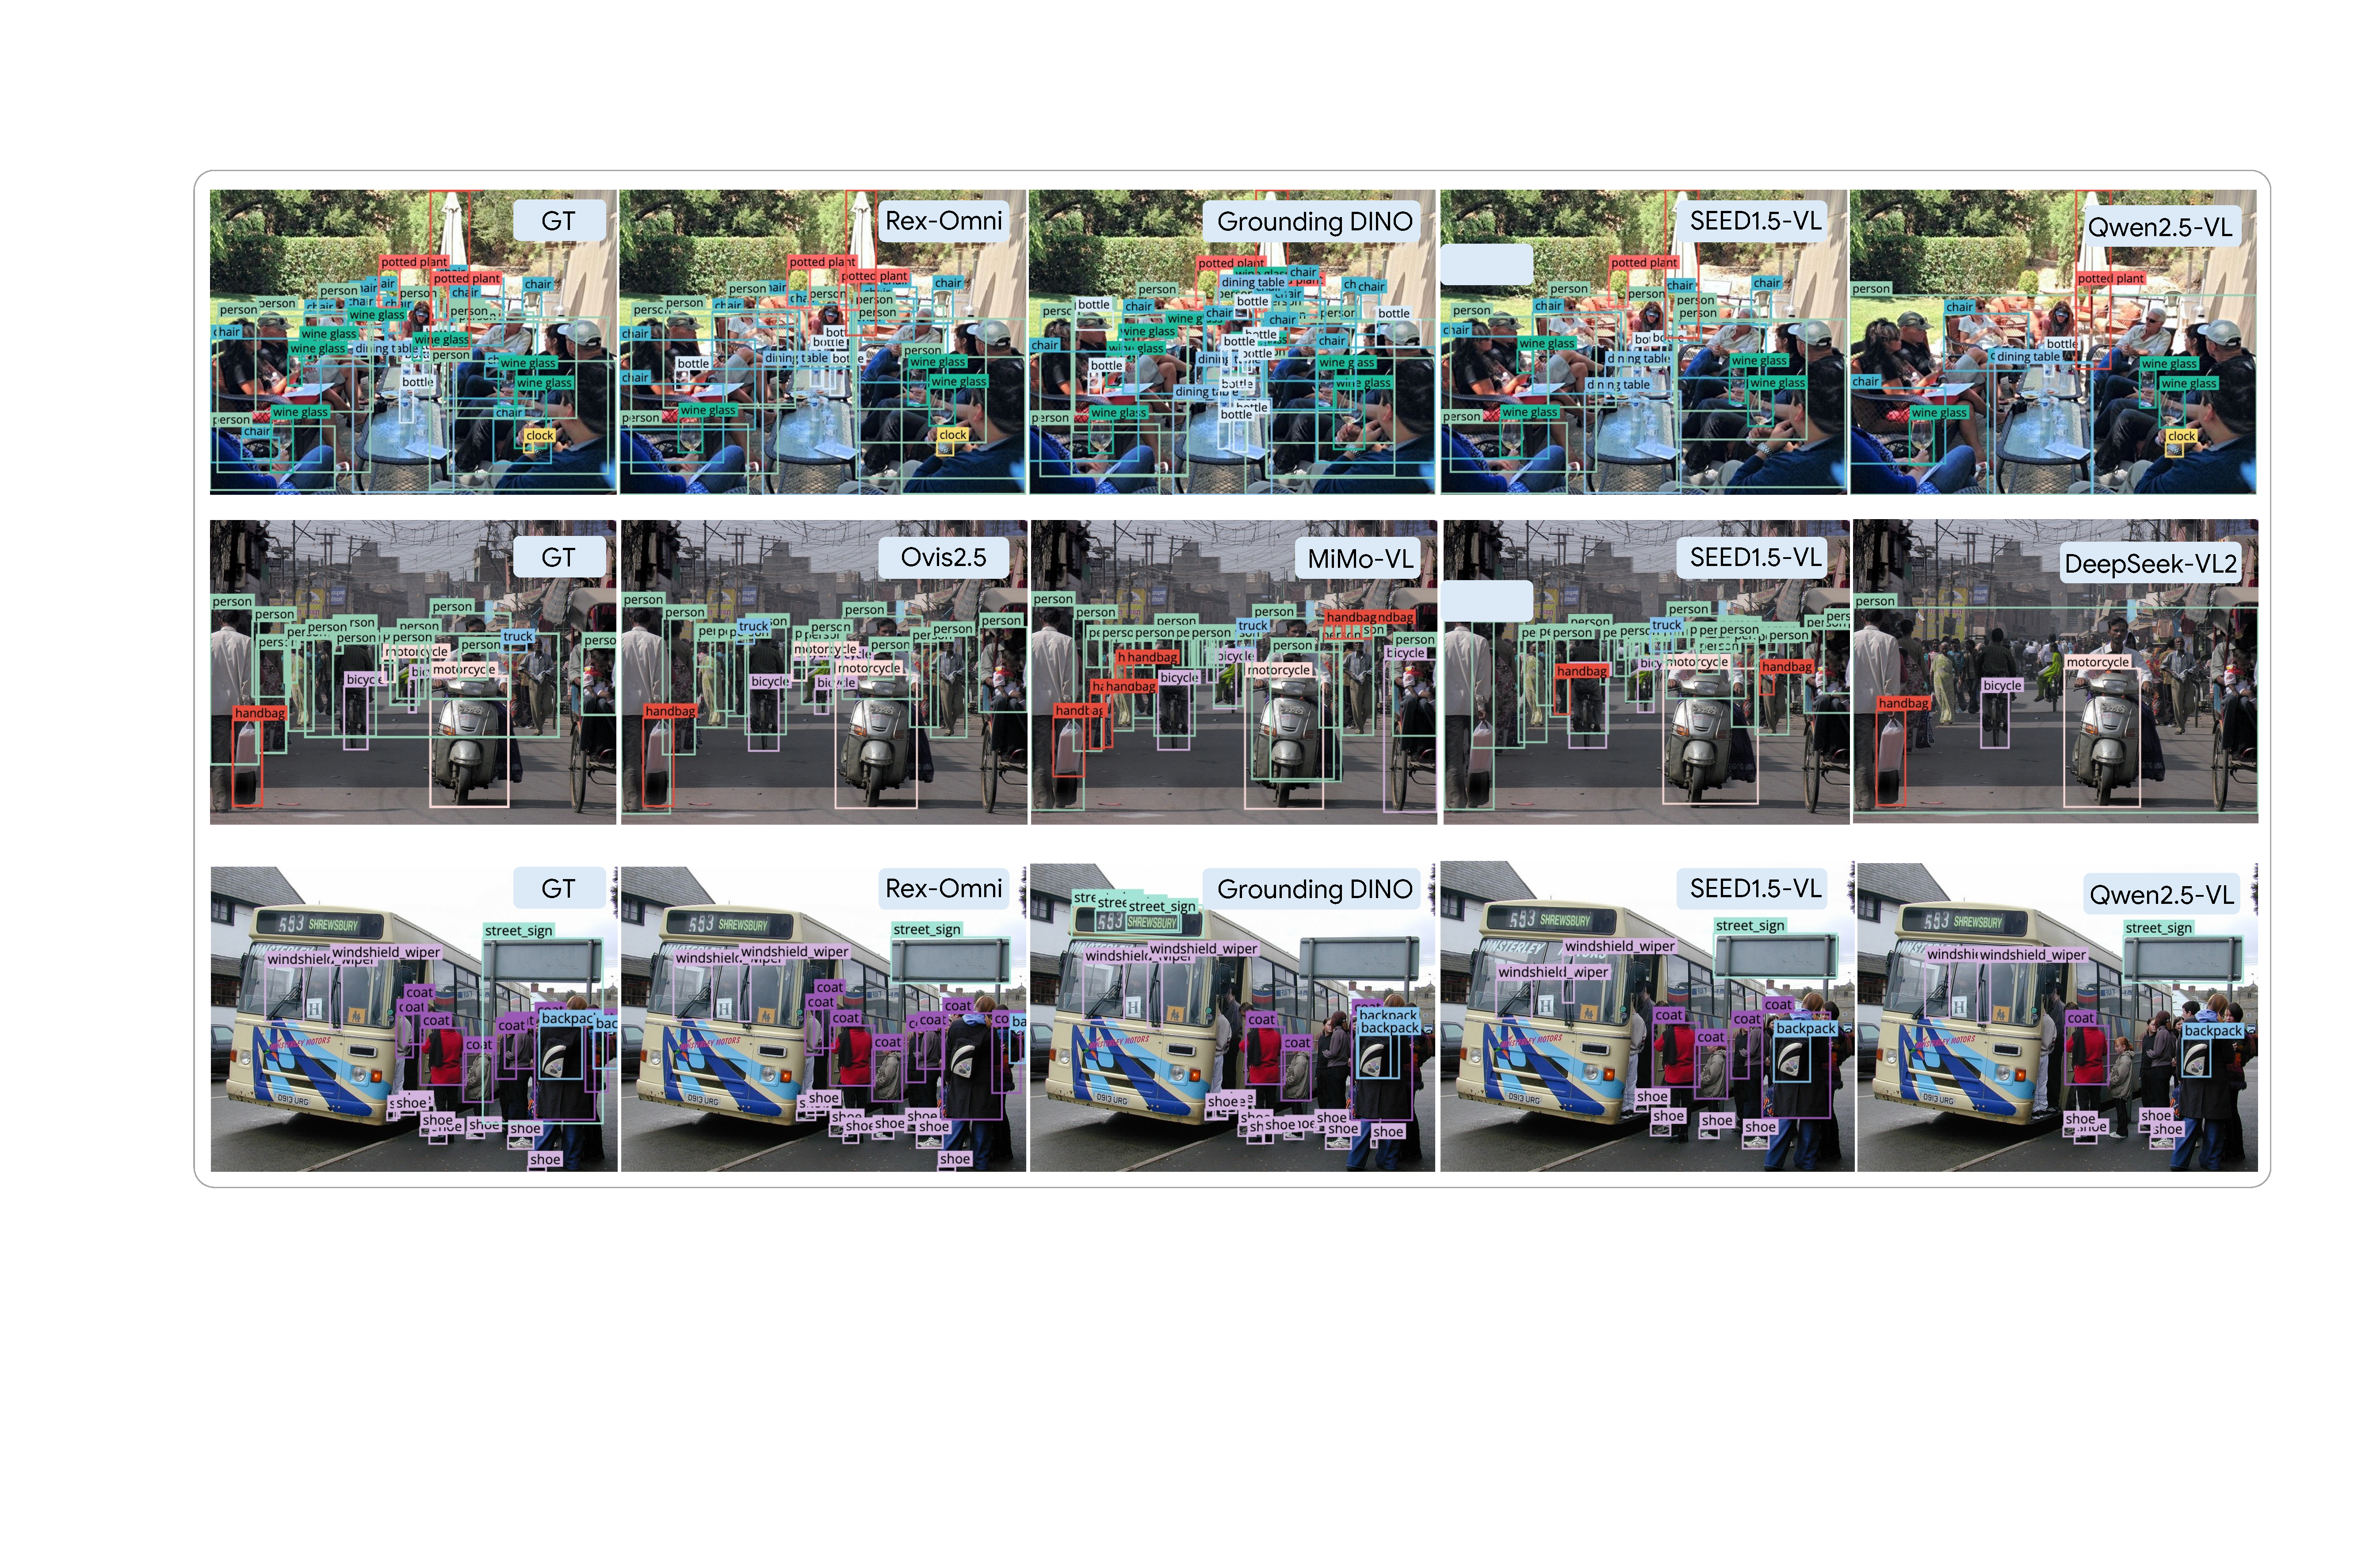
\includegraphics[width=1.0\textwidth]{figures/compare_common_longtail.pdf}
    \caption{Visualization of detection predictions from different models on common and long-tailed object detection benchmarks, using COCO and LVIS, respectively.}
    \label{fig:compare_common_longtail}
\end{figure}

\textbf{Results}: The results are presented in Table \ref{tab:common_object_detection}. Firstly, among MLLMs, Rex-Omni surpasses existing approaches, including SEED1.5-VL, which previously held state-of-the-art detection performance. At an IoU threshold of 0.5, Rex-Omni demonstrates superior performance, outperforming both the open-set detection model Grounding DINO-SwinT and the closed-set detection model DINO-R50. Crucially, Rex-Omni achieves this in a zero-shot setting (without training on COCO data), thereby indicating that MLLM-based detection methods can indeed surpass traditional regression-based models when highly precise bounding box localization is not the sole critical factor. However, at a stricter IoU threshold of 0.95, Rex-Omni's performance, while still strong, only marginally outperforms DAB-DETR, suggesting that MLLMs may still lag behind conventional regression-based models in scenarios demanding extremely precise bounding box tightness.

Nevertheless, despite this nuanced limitation, the achieved performance is generally sufficient for a wide range of practical applications. We show some visualization results in Figure \ref{fig:compare_common_longtail}. Furthermore, a significant improvement is observed with GRPO post-training, where the full Rex-Omni model substantially outperforms its SFT-only variant (Rex-Omni-SFT). This clearly highlights the effectiveness of our reinforcement learning strategy. 

\subsection{Long-tailed Object Detection}
Long-tailed object detection tackles the challenge of recognizing categories with highly imbalanced instance distributions, where most categories are sparsely represented. This task requires models to generalize effectively and robustly detect rare objects in complex real-world scenarios.

\textbf{Benchmark: }We evaluate on the widely used LVIS~\cite{gupta2019lvis} dataset. LVIS comprises 1,203 categories, significantly more than COCO's 80, and features 19,626 test images.  Its categories are derived from WordNet synsets and are intentionally distributed to mimic real-world frequencies, resulting in a natural long-tail distribution where many categories have very few instances. 

\textbf{Evaluation Settings and Metrics: }We assess the performance of open-set detection models and MLLMs, following the same evaluation settings and metrics as described in Section~\ref{sec:coco} for COCO.

\begin{table*}[t]
    \centering
    \resizebox{1.0\textwidth}{!}{
        \begin{tabular}{cc|cc|ccccccccc}
\toprule
\multirow{2}{*}{Type} & \multirow{2}{*}{Method} & \multirow{2}{*}{Zero-Shot} & \multirow{2}{*}{\begin{tabular}[c]{@{}c@{}}Score\\ Thresh.\end{tabular}} & \multicolumn{9}{c}{LVIS} \\
\cline{5-13}
 &  &  &  & \begin{tabular}[c]{@{}c@{}}R@IoU\\ 0.5\end{tabular} & \begin{tabular}[c]{@{}c@{}}P@IoU\\ 0.5\end{tabular} & \multicolumn{1}{c|}{\begin{tabular}[c]{@{}c@{}}F1@IoU\\ 0.5\end{tabular}} & \begin{tabular}[c]{@{}c@{}}R@IoU\\ 0.95\end{tabular} & \begin{tabular}[c]{@{}c@{}}P@IoU\\ 0.95\end{tabular} & \multicolumn{1}{c|}{\begin{tabular}[c]{@{}c@{}}F1@IoU\\ 0.95\end{tabular}} & \begin{tabular}[c]{@{}c@{}}R@\\ mIoU\end{tabular} & \begin{tabular}[c]{@{}c@{}}P@\\ mIoU\end{tabular} & \begin{tabular}[c]{@{}c@{}}F1@\\ mIoU\end{tabular} \\
\midrule
Open-set                & Grounding DINO-Swin-T    & Yes & 0.21 & 39.1 & 61.2 & \multicolumn{1}{c|}{47.7} & 16.9 & \textbf{34.8} & \multicolumn{1}{c|}{\textbf{22.7}} & 31.9 & 49.6 & 38.8 \\
\midrule
\multirow{10}{*}{MLLM}
& DeepSeek-VL2-Tiny        & UNK & - & 22.4 & 55.7 & \multicolumn{1}{c|}{32.0} & 7.2  & 25.7 & \multicolumn{1}{c|}{11.2} & 14.2 & 41.9 & 21.2 \\
& MiMo-VL-7B               & UNK & - & 43.3 & 57.8 & \multicolumn{1}{c|}{49.5} & 6.5  & 13.7 & \multicolumn{1}{c|}{8.8}  & 25.4 & 41.1 & 31.4 \\
& OVIS2.5-2B               & UNK & - & 53.2 & 55.6 & \multicolumn{1}{c|}{54.4} & 13.3 & 19.4 & \multicolumn{1}{c|}{15.8} & 34.0 & 41.6 & 37.4 \\
& OVIS2.5-9B               & UNK & - & 52.2 & 54.1 & \multicolumn{1}{c|}{53.1} & 11.2 & 19.9 & \multicolumn{1}{c|}{14.4} & 32.2 & 40.1 & 35.8 \\
& Qwen2.5-VL-7B            & UNK & - & 47.1 & 74.3 & \multicolumn{1}{c|}{57.7} & 12.7 & 29.0 & \multicolumn{1}{c|}{17.6} & 32.0 & 54.3 & 40.2 \\
& Qwen2.5-VL-3B            & UNK & - & 44.8 & 73.9 & \multicolumn{1}{c|}{55.8} & 14.3 & \underline{29.8} & \multicolumn{1}{c|}{19.3} & 31.9 & 54.6 & 40.3 \\
& DeepSeek-VL2-Small       & UNK & - & 46.1 & 72.2 & \multicolumn{1}{c|}{56.2} & 15.8 & 31.2 & \multicolumn{1}{c|}{\underline{21.0}} & 33.7 & 55.0 & 41.8 \\
& SEED1.5-VL               & Yes & - & \underline{54.7} & \textbf{82.0} & \multicolumn{1}{c|}{\textbf{65.6}} & 15.0 & 28.1 & \multicolumn{1}{c|}{19.5} & \underline{38.5} & \textbf{59.3} & \underline{46.7} \\
\rowcolor{lightblue!10}
& Rex-Omni-SFT             & Yes & - & 52.0 & 71.6 & \multicolumn{1}{c|}{60.3} & \textbf{16.6} & 27.4 & \multicolumn{1}{c|}{20.7} & 37.7 & 53.3 & 44.2 \\
\rowcolor{lightblue!10}
& Rex-Omni                 & Yes & - & \textbf{54.7} & \underline{78.1} & \multicolumn{1}{c|}{\underline{64.3}} & \underline{16.5} & 27.6 & \multicolumn{1}{c|}{20.7} & \textbf{39.6} & \underline{57.5} & \textbf{46.9} \\
\bottomrule
\end{tabular}
    }
    \caption{Performance evaluation on the LVIS dataset for long-tailed object detection. All reported metrics adhere to the same methodology described for COCO evaluation in Section \ref{sec:coco}.}
    \label{tab:long_tailed_object_detection}
\end{table*}


\textbf{Results: }The results are presented in Table~\ref{tab:long_tailed_object_detection}. On LVIS, MLLMs generally outperform traditional open-set detectors such as Grounding DINO, owing to the stronger linguistic reasoning ability of their LLM components compared to conventional text encoders (e.g., CLIP or BERT). This advantage facilitates better generalization to low-frequency categories.

In the zero-shot setting, Rex-Omni achieves competitive performance, with an F1 score at IoU=0.5 second only to SEED1.5-VL, likely due to the latter’s larger model size and stronger language understanding. Notably, Rex-Omni attains state-of-the-art results on the mIoU metric, reflecting its superior bounding box precision across thresholds. Moreover, the substantial improvement from Rex-Omni-SFT to the full Rex-Omni model underscores the effectiveness of GRPO-based reinforcement post-training in enhancing object localization. Qualitative results are shown in Figure~\ref{fig:compare_common_longtail} and Figure~\ref{fig:app_common_longtailed}.

\subsection{Dense and Tiny Object Detection}
\label{sec:dense}
Dense and tiny object detection is crucial for applications such as remote sensing and object counting, requiring accurate localization of numerous small objects in crowded scenes. For MLLMs, this task is particularly challenging: it not only demands precise, extended coordinate predictions sensitive to subtle pixel variations, but also exposes the absence of multi-scale feature mechanisms (e.g., feature pyramids~\cite{lin2017feature}) that traditional regression-based detectors exploit to handle scale diversity. As a result, MLLMs often suffer from issues such as duplicate predictions and coordinate offsets in dense and tiny object detection scenarios.
 
\begin{table*}[t]
    \centering
    \resizebox{1.0\textwidth}{!}{
        \begin{tabular}{cc|c|ccc|ccc}
\toprule
\multirow{2}{*}{Type} & \multirow{2}{*}{Method} & \multirow{2}{*}{\begin{tabular}[c]{@{}c@{}}Score \\ Threshhold\end{tabular}}
& \multicolumn{3}{c|}{Dense200} & \multicolumn{3}{c}{VisDrone} \\
\cline{4-9}
 &  &  & \begin{tabular}[c]{@{}c@{}}F1@IoU\\ 0.5\end{tabular} & \begin{tabular}[c]{@{}c@{}}F1@IoU\\ 0.95\end{tabular} & \begin{tabular}[c]{@{}c@{}}F1@IoU\\ mIoU\end{tabular} & \begin{tabular}[c]{@{}c@{}}F1@IoU\\ 0.5\end{tabular} & \begin{tabular}[c]{@{}c@{}}F1@IoU\\ 0.95\end{tabular} & \begin{tabular}[c]{@{}c@{}}F1@IoU\\ mIoU\end{tabular} \\
\midrule
Open-set & Grounding DINO-Swin-T & 0.25 & 36.9 & \textbf{19.7} & 33.1 & 55.2 & \textbf{3.9} & \textbf{38.5} \\
\midrule
\multirow{10}{*}{MLLM}
& DeepSeek-VL2-Tiny  & - & 2.2  & 0.3 & 1.5 & 4.3  & 0.1 & 1.8 \\
& OVIS2.5-9B         & - & 14.0 & 0.0 & 5.1 & 15.8 & 0.1 & 6.5 \\
& OVIS2.5-2B         & - & 17.9 & 0.0 & 6.7 & 21.0 & 0.1 & 9.2 \\
& MiMo-VL-7B         & - & 29.7 & 0.4 & 15.9 & 27.7 & 0.3 & 14.3 \\
& Qwen2.5-VL-3B      & - & 0.8  & 0.1 & 0.5 & 31.5 & 1.9 & 20.4 \\
& Qwen2.5-VL-7B      & - & 1.1  & 0.1 & 0.6 & 34.5 & 1.6 & 21.7 \\
& DeepSeek-VL2-Small & - & 16.0 & 3.9 & 12.7 & 35.8 & 1.7 & 23.3 \\
& SEED1.5-VL         & - & \underline{76.9} & 5.3 & \underline{53.2} & \underline{55.9} & 0.6 & 27.4 \\
\rowcolor{lightblue!10}
& Rex-Omni-SFT       & - & 60.2 & \underline{10.6} & 46.4 & 55.6 & \underline{1.9} & 32.4 \\
\rowcolor{lightblue!10}
& Rex-Omni           & - & \textbf{78.4} & 10.3 & \textbf{58.3} & \textbf{61.6} & 1.5 & \underline{35.8} \\
\bottomrule
\end{tabular}
    }
    \caption{Evaluation Results on dense object detection benchmark VisDrone and Dense200. We report the same metric used in COCO evaluation at Section \ref{sec:coco}.}
    \label{tab:dense_object_detection}
\end{table*}

\begin{figure}[!h]     
    % \hspace*{-0.05\textwidth}
    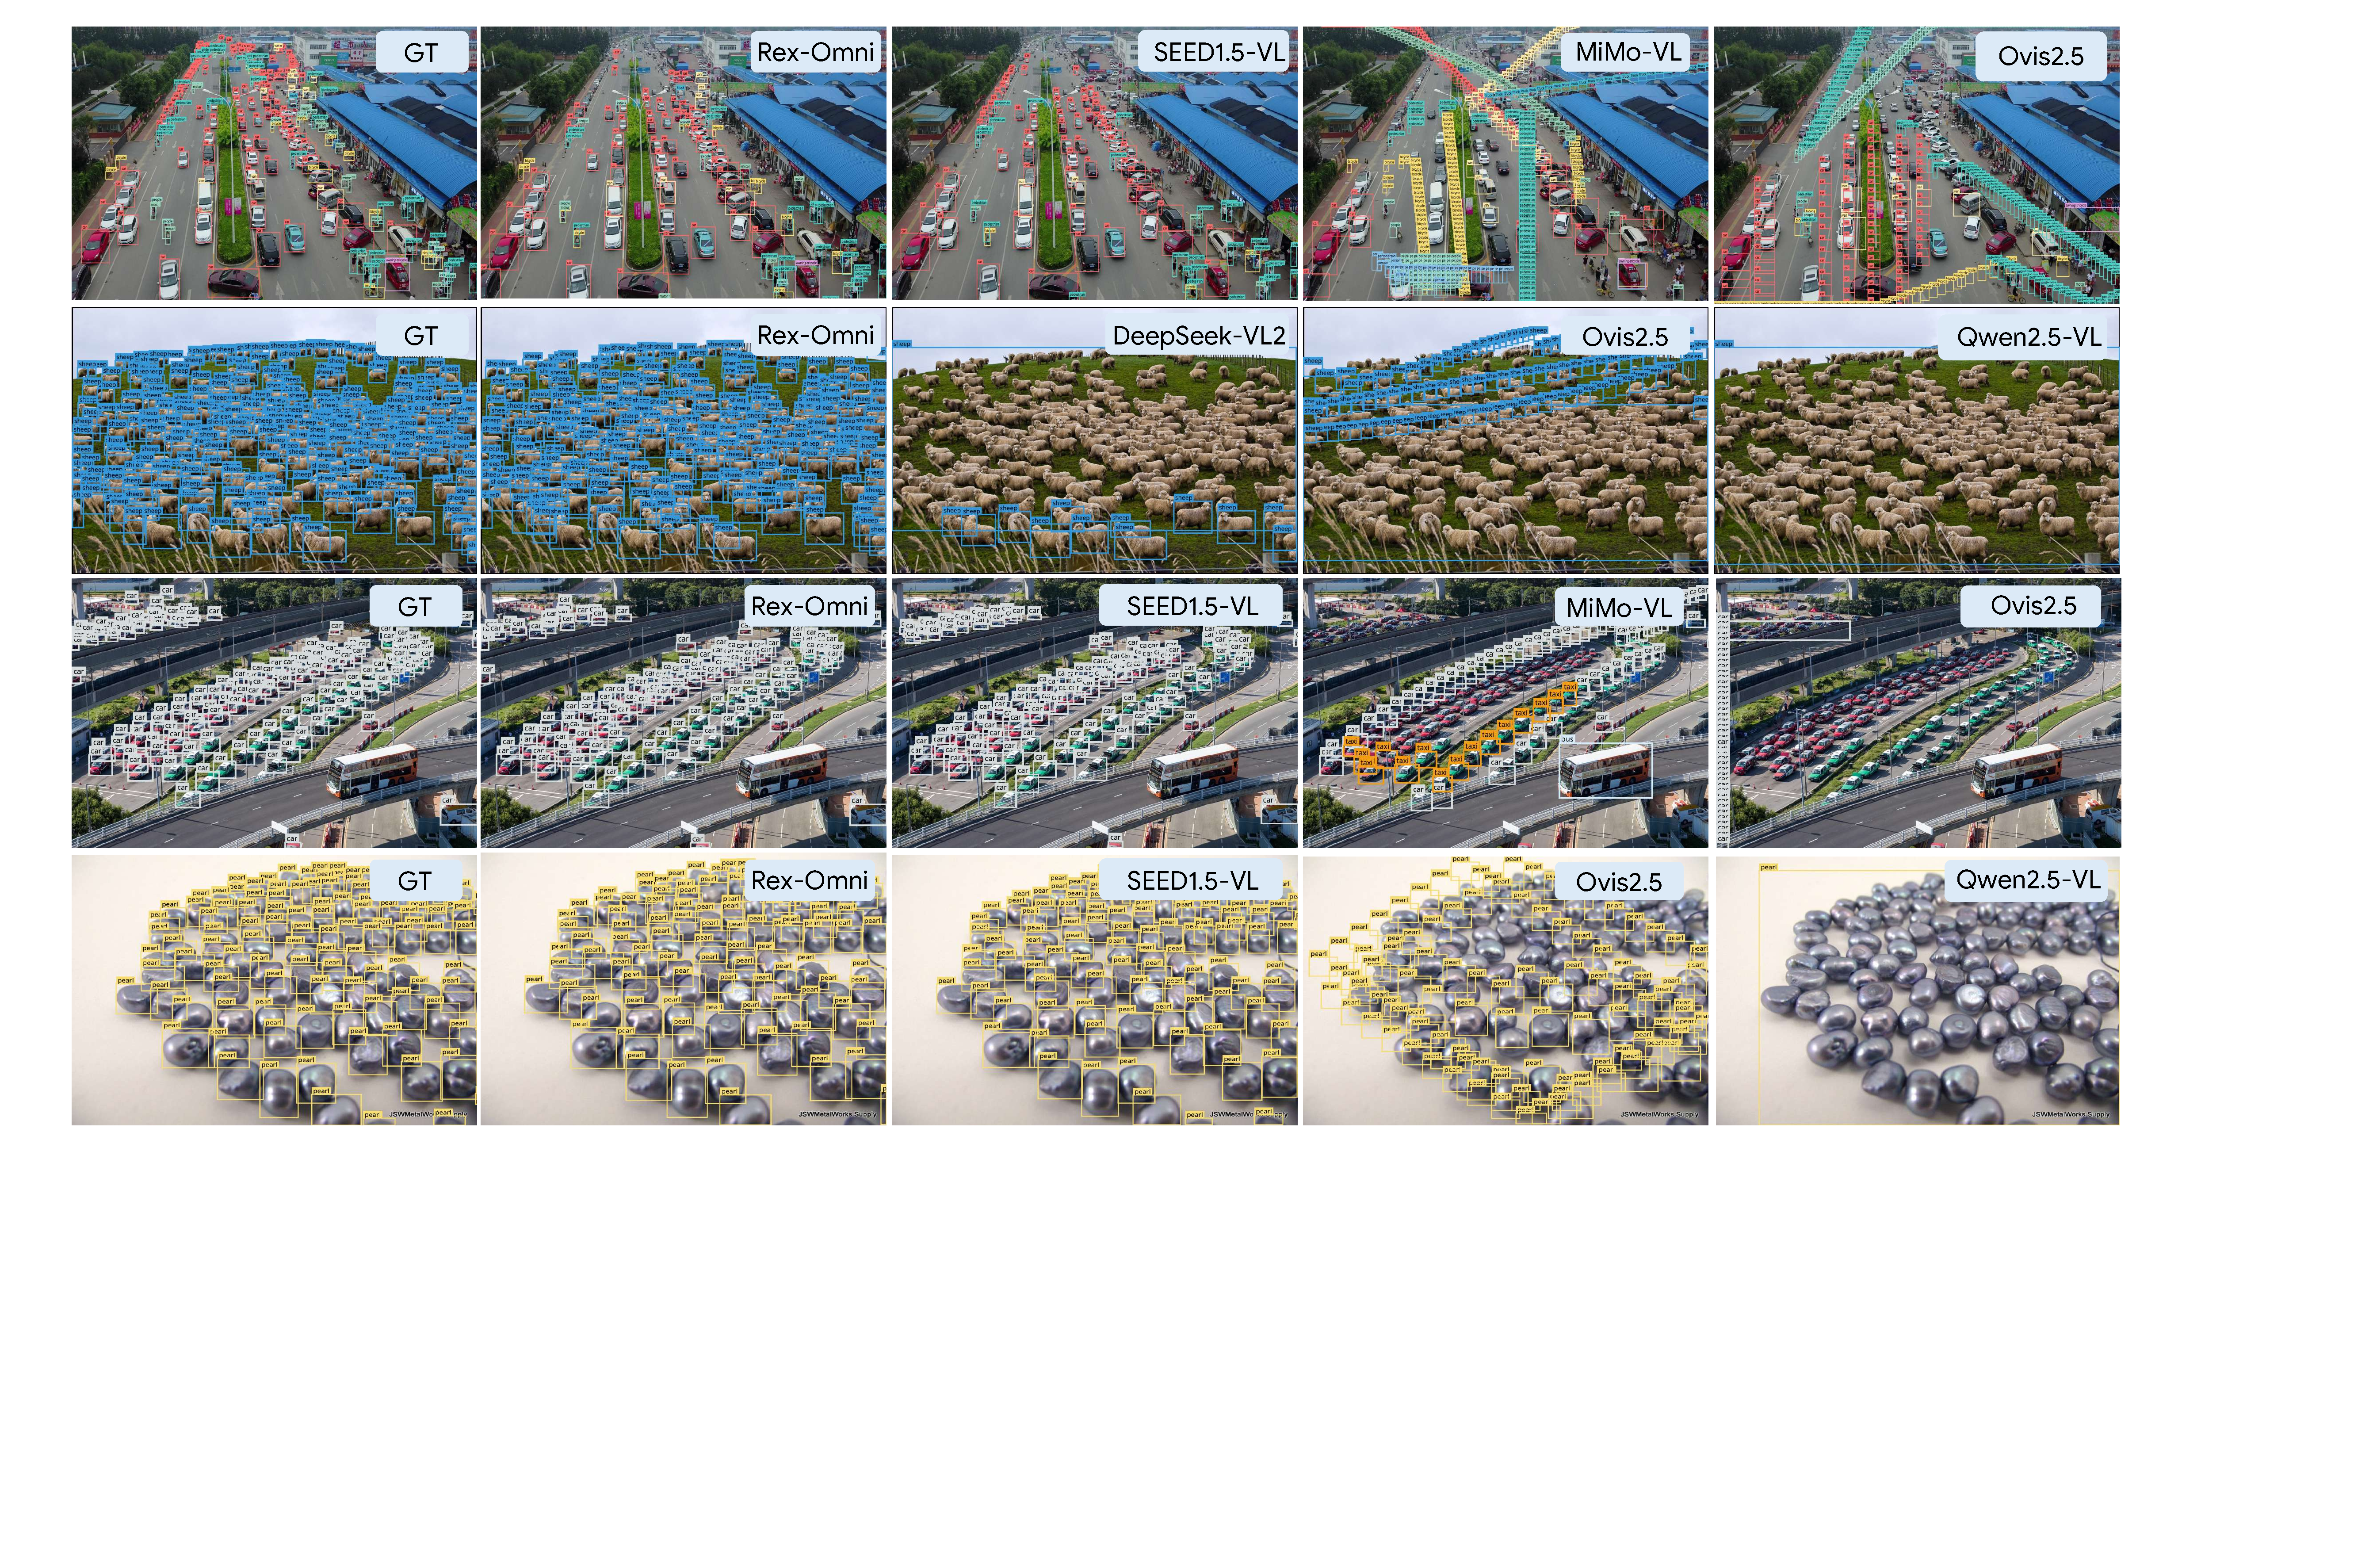
\includegraphics[width=1.0\textwidth]{figures/compare_dense.pdf}
    \caption{Visualization of dense and tiny object detection predictions. This figure presents a qualitative comparison of various models on the VisDrone and Dense200 datasets.}
    \label{fig:compare_dense}
\end{figure}


\noindent\textbf{Benchmark, settings and metrics: }We evaluate open-set detection models and MLLMs on two distinct datasets tailored for dense and tiny object detection. The first dataset, VisDrone~\cite{du2019visdrone}, comprises 1,610 aerial traffic images spanning 10 categories, with individual boxes measuring approximately 30.7×32.4 pixels. Additionally, we introduce Dense200, a manually collected dataset consisting of 200 densely annotated images covering 109 categories. In Dense200, each image contains an average of 91.2 bounding boxes, with an average size of  66.8×64.5 pixels. Together, these datasets pose significant challenges due to the combination of small object sizes and high object density, demanding precise spatial reasoning and accurate localization. The evaluation settings and metrics are the same as those used in Section \ref{sec:coco} for COCO evaluation.

\noindent\textbf{Results}: The results are reported in Table~\ref{tab:dense_object_detection}, with representative visualizations in Figure~\ref{fig:compare_dense} and Figure~\ref{fig:app_dense}. As anticipated in Section \ref{sec:sft_limitation}, MLLMs struggle with dense and tiny object detection, with most models showing poor performance. We identify two critical failure modes: (1) \textbf{Large-box prediction}, where a single oversized bounding box erroneously covers multiple adjacent objects, and (2) \textbf{Structured duplicate predictions}, where repeated coordinates with minimal offsets are generated instead of distinct object boxes.

We attribute these issues to the SFT stage. Teacher-forced training on full ground-truth sequences restricts the model’s ability to regulate its own output structure. Without such guidance at inference, the model fails to decide object counts or avoid redundant predictions. Notably, we also observed these problematic repetitive predictions in our SFT-only variant. Crucially, after GRPO-based reinforcement post-training, these duplication issues largely disappear, compellingly demonstrating the effectiveness of our two-stage pipeline in correcting SFT-induced deficiencies and enabling more coherent, accurate predictions in dense and tiny object scenarios.

\begin{table*}[t]
    \centering
    \resizebox{1.0\textwidth}{!}{
        \begin{tabular}{cc|c|ccc|ccc|ccc}
\toprule
\multirow{2}{*}{Type} & \multirow{2}{*}{Method} & \multirow{2}{*}{\begin{tabular}[c]{@{}c@{}}Score \\ Thresh.\end{tabular}} 
& \multicolumn{3}{c|}{HumanRef} 
& \multicolumn{3}{c|}{RefCOCOg val} 
& \multicolumn{3}{c}{RefCOCOg test} \\
\cline{4-12}
 &  &  & \begin{tabular}[c]{@{}c@{}}F1@IoU\\ 0.5\end{tabular} & \begin{tabular}[c]{@{}c@{}}F1@IoU\\ 0.95\end{tabular} & \begin{tabular}[c]{@{}c@{}}F1@IoU\\ mIoU\end{tabular} 
 & \begin{tabular}[c]{@{}c@{}}F1@IoU\\ 0.5\end{tabular} & \begin{tabular}[c]{@{}c@{}}F1@IoU\\ 0.95\end{tabular} & \begin{tabular}[c]{@{}c@{}}F1@IoU\\ mIoU\end{tabular} 
 & \begin{tabular}[c]{@{}c@{}}F1@IoU\\ 0.5\end{tabular} & \begin{tabular}[c]{@{}c@{}}F1@IoU\\ 0.95\end{tabular} & \begin{tabular}[c]{@{}c@{}}F1@IoU\\ mIoU\end{tabular} \\
\midrule
Open-set & Grounding DINO-Swin-T & 0.25 
& 28.0 & 16.5 & 25.2 
& 52.9 & 20.9 & 45.9 
& 53.8 & 22.9 & 46.8 \\
\midrule
\multirow{10}{*}{MLLM}
& DeepSeek-VL2-Tiny & - 
& 39.1 & 16.9 & 31.4 
& 67.4 & 16.1 & 50.5 
& 69.3 & 16.9 & 52.1 \\
& OVIS2.5-2B & - 
& 70.6 & 12.3 & 50.0 
& 87.4 & 29.3 & 73.4 
& 87.6 & 30.5 & 73.8 \\
& OVIS2.5-9B & - 
& 73.1 & 12.4 & 52.8 
& \underline{88.8} & 23.5 & 72.1 
& \textbf{88.7} & 24.2 & 72.6 \\
& Qwen2.5-VL-3B & - 
& 66.7 & 46.8 & 60.5 
& 83.5 & 30.7 & 69.2 
& 83.8 & 31.8 & 70.1 \\
& MiMo-VL-7B & - 
& 77.6 & 26.4 & 63.4 
& 84.9 & 14.4 & 65.3 
& 84.6 & 14.9 & 65.5 \\
& Qwen2.5-VL-7B & - 
& 72.9 & 42.9 & 64.1 
& 86.2 & 27.2 & 70.0 
& 85.7 & 28.4 & 70.4 \\
& DeepSeek-VL2-Small & - 
& 72.0 & 46.5 & 64.7 
& \textbf{92.4} & \textbf{45.6} & \textbf{81.4} 
& \textbf{91.8} & \textbf{47.0} & \textbf{81.6} \\
& SEED1.5-VL & - 
& \textbf{88.2} & 60.0 & \textbf{81.6} 
& 84.7 & 30.9 & 71.9 
& 85.2 & 32.1 & 73.2 \\
\rowcolor{lightblue!10}
& Rex-Omni-SFT & - 
& 83.3 & \underline{64.3} & 77.9 
& 84.9 & 34.2 & 71.7 
& 85.2 & 35.2 & 72.4 \\
\rowcolor{lightblue!10}
& Rex-Omni & - 
& \underline{85.4} & \textbf{65.4} & \underline{79.9} 
& 86.6 & \underline{35.3} & \underline{73.6} 
& 86.8 & \underline{36.6} & \underline{74.3} \\
\bottomrule
\end{tabular}
    }
    \caption{Evaluation results on referring expression comprehension benchmarks, including HumanRef and RefCOCOg.}
    \label{tab:referring_detection}
\end{table*}

\begin{figure}[!h]     
    % \hspace*{-0.05\textwidth}
    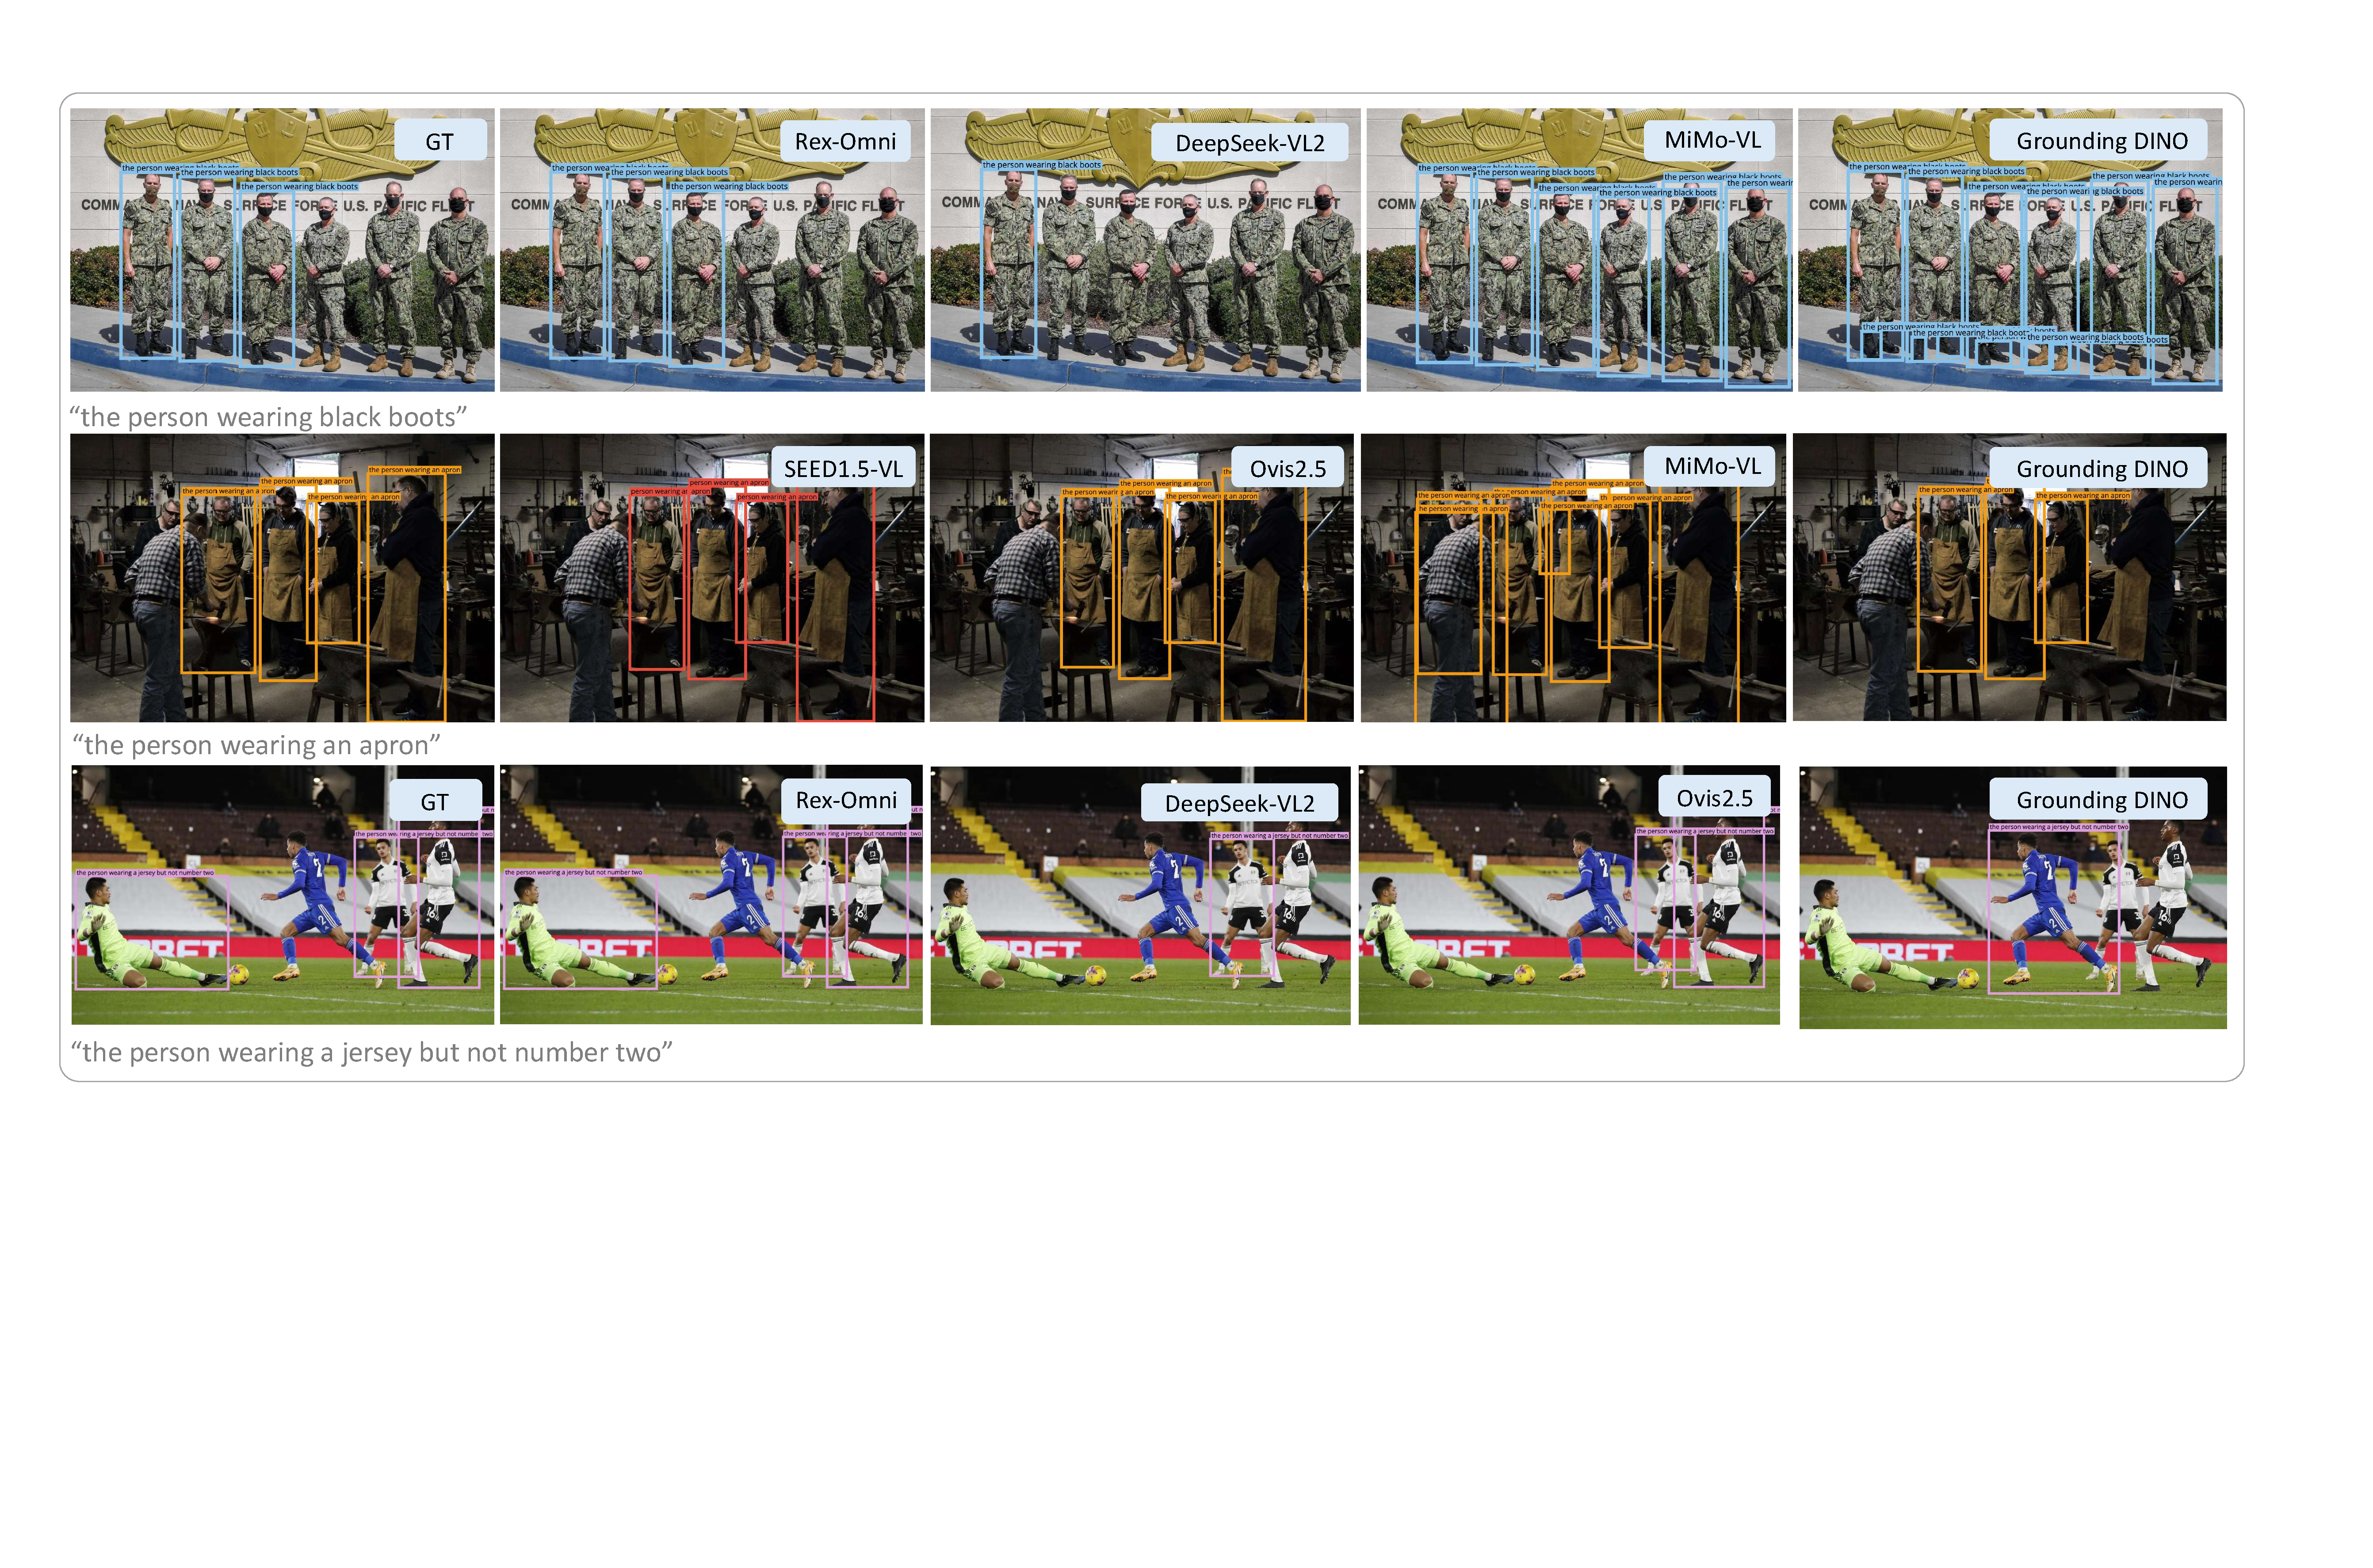
\includegraphics[width=1.0\textwidth]{figures/referring_comparsion.pdf}
    \captionsetup{justification=centering}
    \caption{Visualization of model predictions on referring object detection benchmarks.}
    \label{fig:compare_referring}
\end{figure}


\subsection{Referring Object Detection}
Referring object detection requires a model to identify and localize objects described by a natural language expression. Unlike standard object detection, which focuses on category-level recognition, this task demands fine-grained language understanding and strong alignment between linguistic descriptions and visual content.

\textbf{Benchmark: }The evaluation is conducted on two established public benchmarks:
\textbf{1) RefCOCOg (val/test):} RefCOCOg~\cite{Datasets:REFCOCOG} is built on COCO images and includes 4,889 validation and 9,577 test referring expressions. Each expression maps to a single ground-truth bounding box, making this benchmark relatively straightforward for evaluation.
\textbf{2) HumanRef:} HumanRef~\cite{jiang2025referringperson} is a human-annotated benchmark focused on people, comprising 6,000 test expressions organized into six subsets: attribute, position, interaction, reasoning, celebrity, and rejection. We use the first five subsets (5,000 images) for evaluation. Unlike RefCOCOg, a single expression in HumanRef may correspond to multiple ground-truth boxes, averaging two per expression. This design poses greater challenges, requiring both fine-grained language understanding and robust visual perception.

\textbf{Evaluation Settings and Metrics}: We evaluate open-set detection models and MLLMs using the same settings and metrics as in Section~\ref{sec:coco} for COCO, with one exception: during testing, models are queried with a single referring expression at a time. For the open-set detector Grounding DINO, we adopt its official demo confidence threshold of 0.25

\textbf{Results}: The results are presented in Table \ref{tab:referring_detection}. Open-set detection models notably struggle with this task, as evidenced by Grounding DINO’s consistent underperformance across benchmarks. In stark contrast, MLLMs, leveraging their inherent strong language understanding capabilities, consistently excel at this task. On HumanRef, Rex-Omni achieves competitive results, ranking second only to SEED1.5-VL. This indicates that, while Rex-Omni (3B parameters) possesses sufficient language understanding for effective REC, larger models like SEED1.5-VL benefit from greater capacity for more nuanced reasoning. Overall, Rex-Omni’s strong performance across all datasets demonstrates its ability to align natural language with visual content, making it highly practical for real-world referring scenarios. Visualization examples are shown in Figure~\ref{fig:compare_referring} and and Figure~\ref{fig:app_referring}.

% \subsection{Hallucination Rejection}

% \input{tables/rejection}
% \begin{figure}[t]     
%     \centering
%     % \hspace*{-0.05\textwidth}
%     \includegraphics[width=0.9\textwidth]{figures/comparsion_rejection.pdf}
%     \caption{Visualization of hallucination examples. The figure illustrates erroneous predictions made by MLLMs for non-existent objects, where models generate bounding boxes despite the absence of corresponding visual content.}
%     \label{fig:compare_rejection}
% \end{figure}

% Beyond accurately detecting existent objects, a truly robust model must also refrain from predicting objects when the input prompt lacks corresponding visual content. In this section, we evaluate a model's ability to reject hallucinations, specifically its capacity to avoid generating coordinates for non-existent objects.

% \textbf{Benchmarks and Evaluation Settings: }
% To evaluate hallucination rejection, we construct specific rejection benchmarks from the COCO and LVIS datasets. Specifically, for each test image, a category not present in that image is randomly sampled from the full set of dataset categories and used as the rejection prompt. The model is then queried with this category, and its capacity to refrain from producing any predictions is measured.

% \textbf{Metrics}
% The rejection rate is employed as the primary evaluation metric. For a given test sample, the model is considered to have correctly rejected a hallucination if it outputs no coordinates. The rejection rate is computed as the proportion of correctly rejected instances out of the total number of test instances.

% \textbf{Results:}
% The experimental results are summarized in Table \ref{tab:rejection}. The experiments reveal that several existing MLLMs, alongside Grounding DINO, exhibit severe hallucination, frequently predicting coordinates for objects entirely absent from the image. Figure \ref{fig:compare_rejection} visualizes representative examples of these erroneous predictions.

% We attribute this deficiency in rejection capability to the absence of negative samples during coordinate prediction training. To verify this hypothesis, we conducted an ablation study on Rex-Omni, comparing models trained with and without randomly sampled negative prompts. The results clearly demonstrate that when negative samples are not included in training, Rex-Omni fails to reject non-existent objects, yielding a rejection score of 0 on both COCO and LVIS. This finding underscores the inherent tendency of MLLMs to overfit training patterns. Based on this critical observation, our final Rex-Omni training pipeline incorporates negative prompt sampling, which effectively enables the model to correctly withhold predictions when prompted with non-existent objects.
\begin{table*}[t]
    \centering
    \resizebox{\textwidth}{!}{
       \begin{tabular}{c|c|cccc|cccc|cccc|cccc}
\toprule
\multirow{2}{*}{Type} & \multirow{2}{*}{Method} 
& \multicolumn{4}{c|}{FSC147-test} 
& \multicolumn{4}{c|}{Dense200} 
& \multicolumn{4}{c|}{COCO} 
& \multicolumn{4}{c}{LVIS} \\ 
\cline{3-18}
 &  & \begin{tabular}[c]{@{}c@{}}F1@\\ 0.5\end{tabular} 
 & \begin{tabular}[c]{@{}c@{}}F1@\\ 0.95\end{tabular} 
 & \begin{tabular}[c]{@{}c@{}}F1@\\ mIoU\end{tabular} 
 & MAE 
 & \begin{tabular}[c]{@{}c@{}}F1@\\ 0.5\end{tabular} 
 & \begin{tabular}[c]{@{}c@{}}F1@\\ 0.95\end{tabular} 
 & \begin{tabular}[c]{@{}c@{}}F1@\\ mIoU\end{tabular} 
 & MAE 
 & \begin{tabular}[c]{@{}c@{}}F1@\\ 0.5\end{tabular} 
 & \begin{tabular}[c]{@{}c@{}}F1@\\ 0.95\end{tabular} 
 & \begin{tabular}[c]{@{}c@{}}F1@\\ mIoU\end{tabular} 
 & MAE 
 & \begin{tabular}[c]{@{}c@{}}F1@\\ 0.5\end{tabular} 
 & \begin{tabular}[c]{@{}c@{}}F1@\\ 0.95\end{tabular} 
 & \begin{tabular}[c]{@{}c@{}}F1@\\ mIoU\end{tabular} 
 & MAE \\ 
\midrule
\multirow{3}{*}{Counting} 
& BMNet+~\cite{shi2022representcomparelearnsimilarityaware} & - & - & - & 14.6 & - & - & - & - & - & - & - & - & - & - & - & - \\
& CountTR~\cite{liu2023countrtransformerbasedgeneralisedvisual} & - & - & - & 12.0 & - & - & - & - & - & - & - & - & - & - & - & - \\
& DAVE~\cite{pelhan2024davedetectandverifyparadigm} & - & - & - & 8.7 & - & - & - & - & - & - & - & - & - & - & - & - \\
\midrule
Open-set 
& T-Rex2~\cite{jiang2024t} 
& \textbf{91.5} & \textbf{47.5} & \textbf{73.3} & 10.9 
& \textbf{93.9} & \textbf{67.1} & \textbf{88.1} & \textbf{6.5} 
& 72.3 & \textbf{19.9} & 57.8 & \textbf{4.0} 
& \underline{71.1} & \textbf{34.6} & \textbf{58.8} & \textbf{3.4} \\
\midrule
\multirow{2}{*}{MLLM} & \cellcolor{lightblue!10} Rex-Omni-SFT 
& \cellcolor{lightblue!10}\underline{87.0} &\cellcolor{lightblue!10} \cellcolor{lightblue!10}\underline{10.5} & \cellcolor{lightblue!10}\underline{64.6} & \cellcolor{lightblue!10}\underline{7.8} 
& \cellcolor{lightblue!10}65.1 & \cellcolor{lightblue!10}11.1 &\cellcolor{lightblue!10} 50.0 &\cellcolor{lightblue!10} 50.9 
&\cellcolor{lightblue!10} \underline{73.6} & \cellcolor{lightblue!10}\underline{19.8} & \cellcolor{lightblue!10}\underline{58.4} &\cellcolor{lightblue!10} 11.7 
& \cellcolor{lightblue!10}70.2 & \cellcolor{lightblue!10}\underline{26.3} & \cellcolor{lightblue!10}56.0 &\cellcolor{lightblue!10} 11.7 \\
 & \cellcolor{lightblue!10}Rex-Omni 
& \cellcolor{lightblue!10}86.0 & \cellcolor{lightblue!10}10.5 & \cellcolor{lightblue!10}62.8 & \cellcolor{lightblue!10}\textbf{7.0} 
& \cellcolor{lightblue!10}\underline{79.5} & \cellcolor{lightblue!10}\underline{10.8} & \cellcolor{lightblue!10}\underline{59.2} & \cellcolor{lightblue!10}\underline{20.1} 
& \cellcolor{lightblue!10}\textbf{79.1} & \cellcolor{lightblue!10}19.4 & \cellcolor{lightblue!10}\textbf{61.3} & \cellcolor{lightblue!10}\underline{4.5} 
& \cellcolor{lightblue!10}\textbf{74.4} & \cellcolor{lightblue!10}24.8 & \cellcolor{lightblue!10}\underline{57.0} & \cellcolor{lightblue!10}\underline{5.2} \\
\bottomrule
\end{tabular}
    }
    \caption{Evaluation results for the visual prompting task across COCO, LVIS, Dense200, and FSC147 datasets. Performance is assessed using F1-score for detection and Mean Absolute Error (MAE) for object counting.}
    \label{tab:visual_prompting}
\end{table*}



\subsection{Visual Prompting}

While text prompts are widely used in many tasks, they have inherent limitations, particularly when certain objects are difficult to describe using language alone. In such scenarios, visual prompting can offer a more effective approach for object detection. In this section, we define visual prompting as a task where, given an image alongside several example bounding boxes within it, the model is required to detect all other objects belonging to the same category as those indicated by the examples.

\textbf{Benchmark and Evaluation Setting:}
We evaluate visual prompting on the object counting dataset FSC147~\cite{ranjan2021learning}, as well as on object detection benchmarks COCO, LVIS, and Dense200. The FSC147 dataset consists of 1,190 images, each containing a dense set of objects from a single category along with three example bounding boxes, which are used as visual prompts for detection. For COCO, LVIS, and Dense200, we follow the T-Rex2~\cite{jiang2024t} methodology, where for each ground-truth category in an image, one bounding box is randomly sampled as the visual prompt for that category. To interface with Rex-Omni, the coordinates of the selected visual prompt box are converted into special tokens and embedded into the query, e.g., “Given reference boxes <12><52><212><337> indicating one or more objects, find all objects of the same category in the image.”


\textbf{Metric:}
We primarily adopt the F1-score as described in Section~\ref{sec:coco} for object detection. Additionally, we introduce the Mean Absolute Error (MAE) metric to evaluate the model’s object counting ability. MAE is computed as the absolute difference between predicted and ground-truth object counts, averaged across the entire dataset, thereby providing an additional measure of the model’s capability to accurately count objects in dense scenes.

\textbf{Results:}
While Rex-Omni’s overall performance still falls short of the traditional expert model T-Rex2, it demonstrates strong visual prompting capabilities. In particular, Rex-Omni performs well in both dense scenes and long-tailed scenarios, highlighting its effectiveness in addressing high object density and severe class imbalance. Representative visualization results are shown in Figure~\ref{fig:compare_visual_prompt}.

\begin{figure}[!h]     
    \centering
    % \hspace*{-0.05\textwidth}
    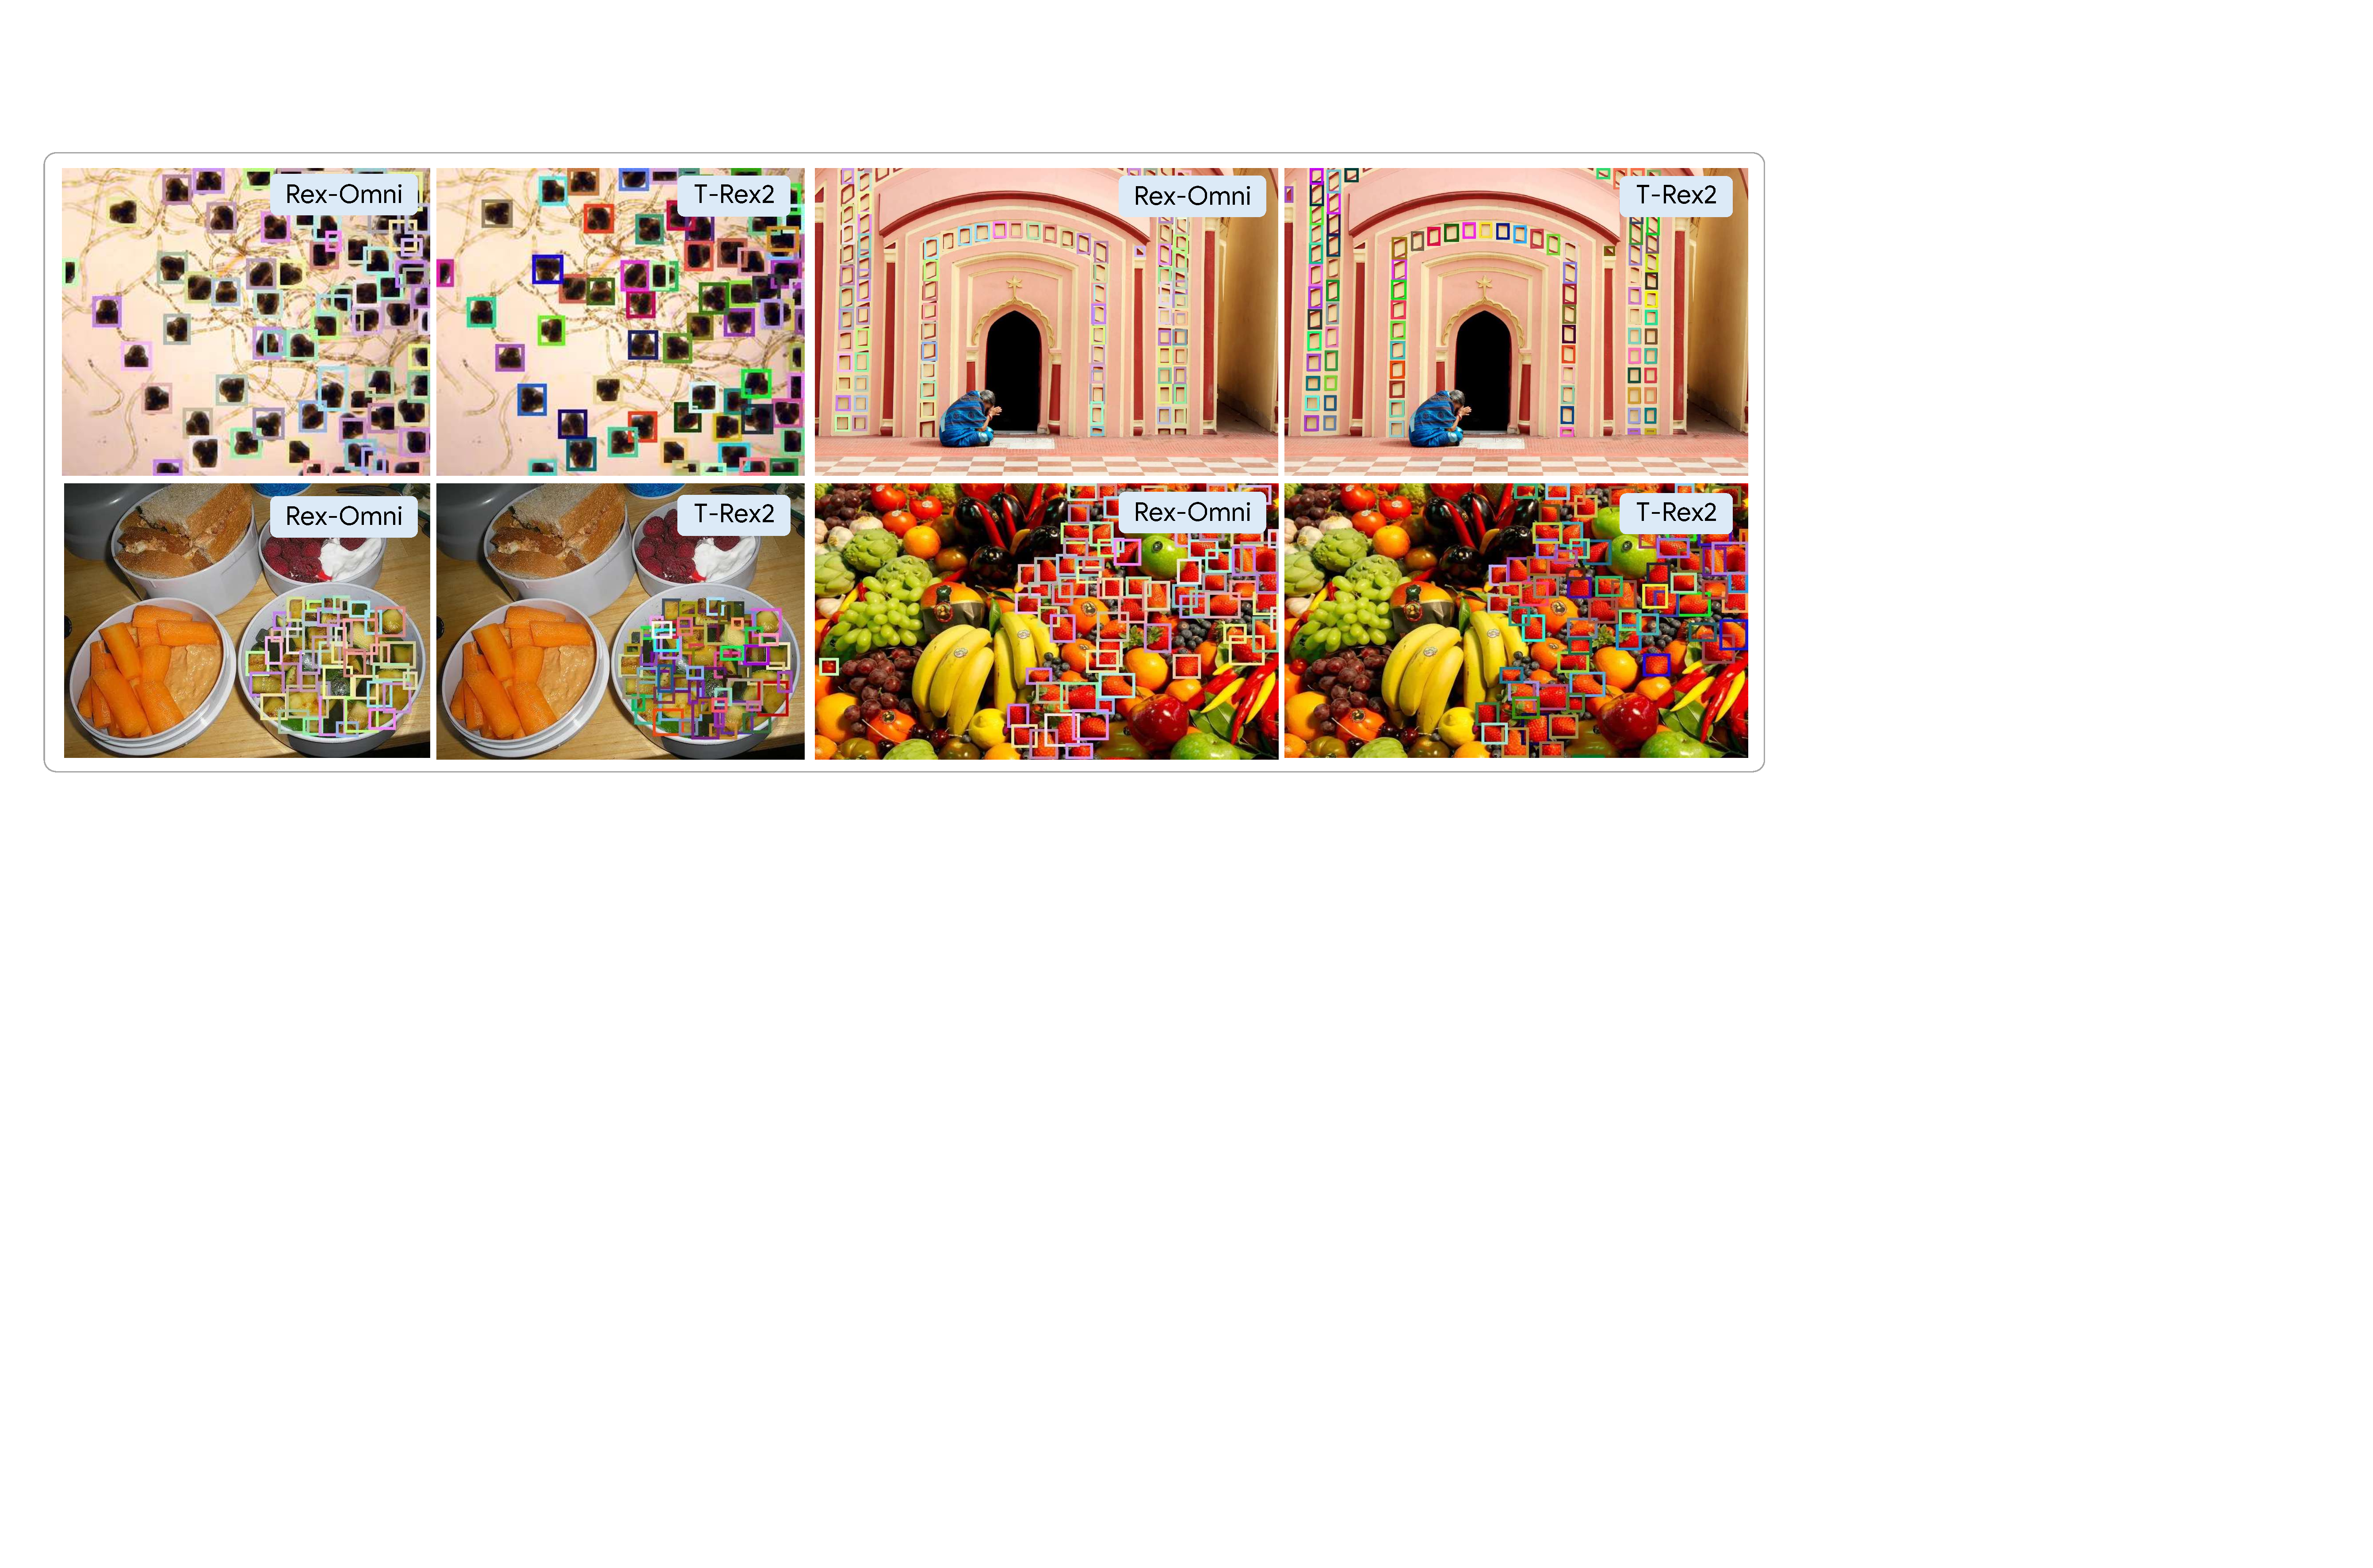
\includegraphics[width=\textwidth]{figures/compare_visual_prompt.pdf}
    \captionsetup{justification=centering}
    \caption{Qualitative comparison of visual prompting predictions between T-Rex2 and Rex-Omni.}
    \label{fig:compare_visual_prompt}
\end{figure}

\subsection{Object Pointing}
The object pointing task requires models to predict precise point coordinates for specified target objects. Unlike bounding boxes, point annotations offer greater flexibility in localization, as models can indicate an object’s center or any representative position within its boundaries.

\textbf{Benchmarks, Evaluation Settings and Metric: }To evaluate object pointing, we integrate datasets previously used for box-based detection, including COCO, LVIS, Dense200, VisDrone, RefCOCOg, and HumanRef. This collection covers a broad range of visual scenarios, from common and long-tailed objects to dense small objects and complex referring expressions. The evaluation protocol follows that of the earlier detection tasks. For most models, except SEED1.5-VL and Rex-Omni, each test image is queried with a single ground-truth category at a time. We adopt the same F1-score–based evaluation metric as in object detection, with one modification in the matching criterion. For each ground-truth bounding box, we generate a segmentation mask using SAM, and a predicted point is considered correct if it falls within the corresponding mask. Recall, Precision, and F1 are then computed analogously to standard box-based evaluation.

\begin{table*}[t]
    \centering
    \resizebox{1.0\textwidth}{!}{
       \begin{tabular}{c|cc|cc|ccc}
\toprule
                         & COCO                              & LVIS                              & Dense200                    & VisDrone      & HumanRef      & RefCOCOg val  & RefCOCOg test \\ \cline{2-8} 
\multirow{-2}{*}{Method} & F1@Point                          & F1@Point                          & F1@Point                    & F1@Point      & F1@Point      & F1@Point      & F1@Point      \\ \midrule
OVIS2.5-2B               & 73.4                              & 52.8                              & 36.4                        & 23.8          & 72.5          & 83.1          & 83.1          \\
Qwen2.5-VL-3B            & 65.9                              & 48.3                              & 4.3                         & 13.9          & 64.1          & 77.4          & 77.8          \\
Qwen2.5-VL-7B            & 61.1                              & 56.5                              & 2.0                         & 14.2          & 65.1          & 78.9          & 79.4          \\
OVIS2.5-9B               & 72.6                              & 61.7                              & 35.0                        & 18.8          & 62.3          & \textbf{85.0} & {\underline{84.5}}    \\
Molmo-7B-D               & 77.3                              & 40.3                              & 33.1                        & 29.2          & 70.0          & 83.7          & 83.6          \\
SEED1.5-VL               & {\color[HTML]{000000} {\underline{78.2}}} & {\color[HTML]{000000} {\underline{70.7}}} & {\color[HTML]{000000} 72.1} & {\underline{56.7}}    & {\underline{83.1}}    & 83.6          & 84.2          \\
  \rowcolor{lightblue!10}  Rex-Omni-SFT             & 76.0                              & 66.7                              & {\underline{72.9}}                  & 49.5          & 82.1          & 83.3          & 83.9          \\
 \rowcolor{lightblue!10} Rex-Omni                 & \textbf{80.5}                     & \textbf{70.8}                     & \textbf{82.5}               & \textbf{58.9} & \textbf{83.8} & {\underline{84.7}}    & \textbf{85.1} \\ \bottomrule
\end{tabular}
    }
    \centering
    \caption{Performance evaluation for the object pointing task across a diverse range of benchmarks (COCO, LVIS, Dense200, VisDrone, RefCOCOg, HumanRef). F1-scores are used as the primary metric.}
    \label{tab:pointing}
    \vspace{-1em}
\end{table*}

\textbf{Results: }The performance of all evaluated models is reported in Table~\ref{tab:pointing}. While most MLLMs achieve reasonable pointing accuracy on common object categories, they struggle with dense or small-scale instances, particularly on Dense200 and VisDrone. Rex-Omni attains the highest F1-scores across both general and challenging datasets, highlighting its strong spatial localization ability. Representative visualizations are shown in Figure~\ref{fig:compare_pointing} and and Figure~\ref{fig:app_pointing}.

\begin{figure}[t]     
    \centering
    % \hspace*{-0.05\textwidth}
    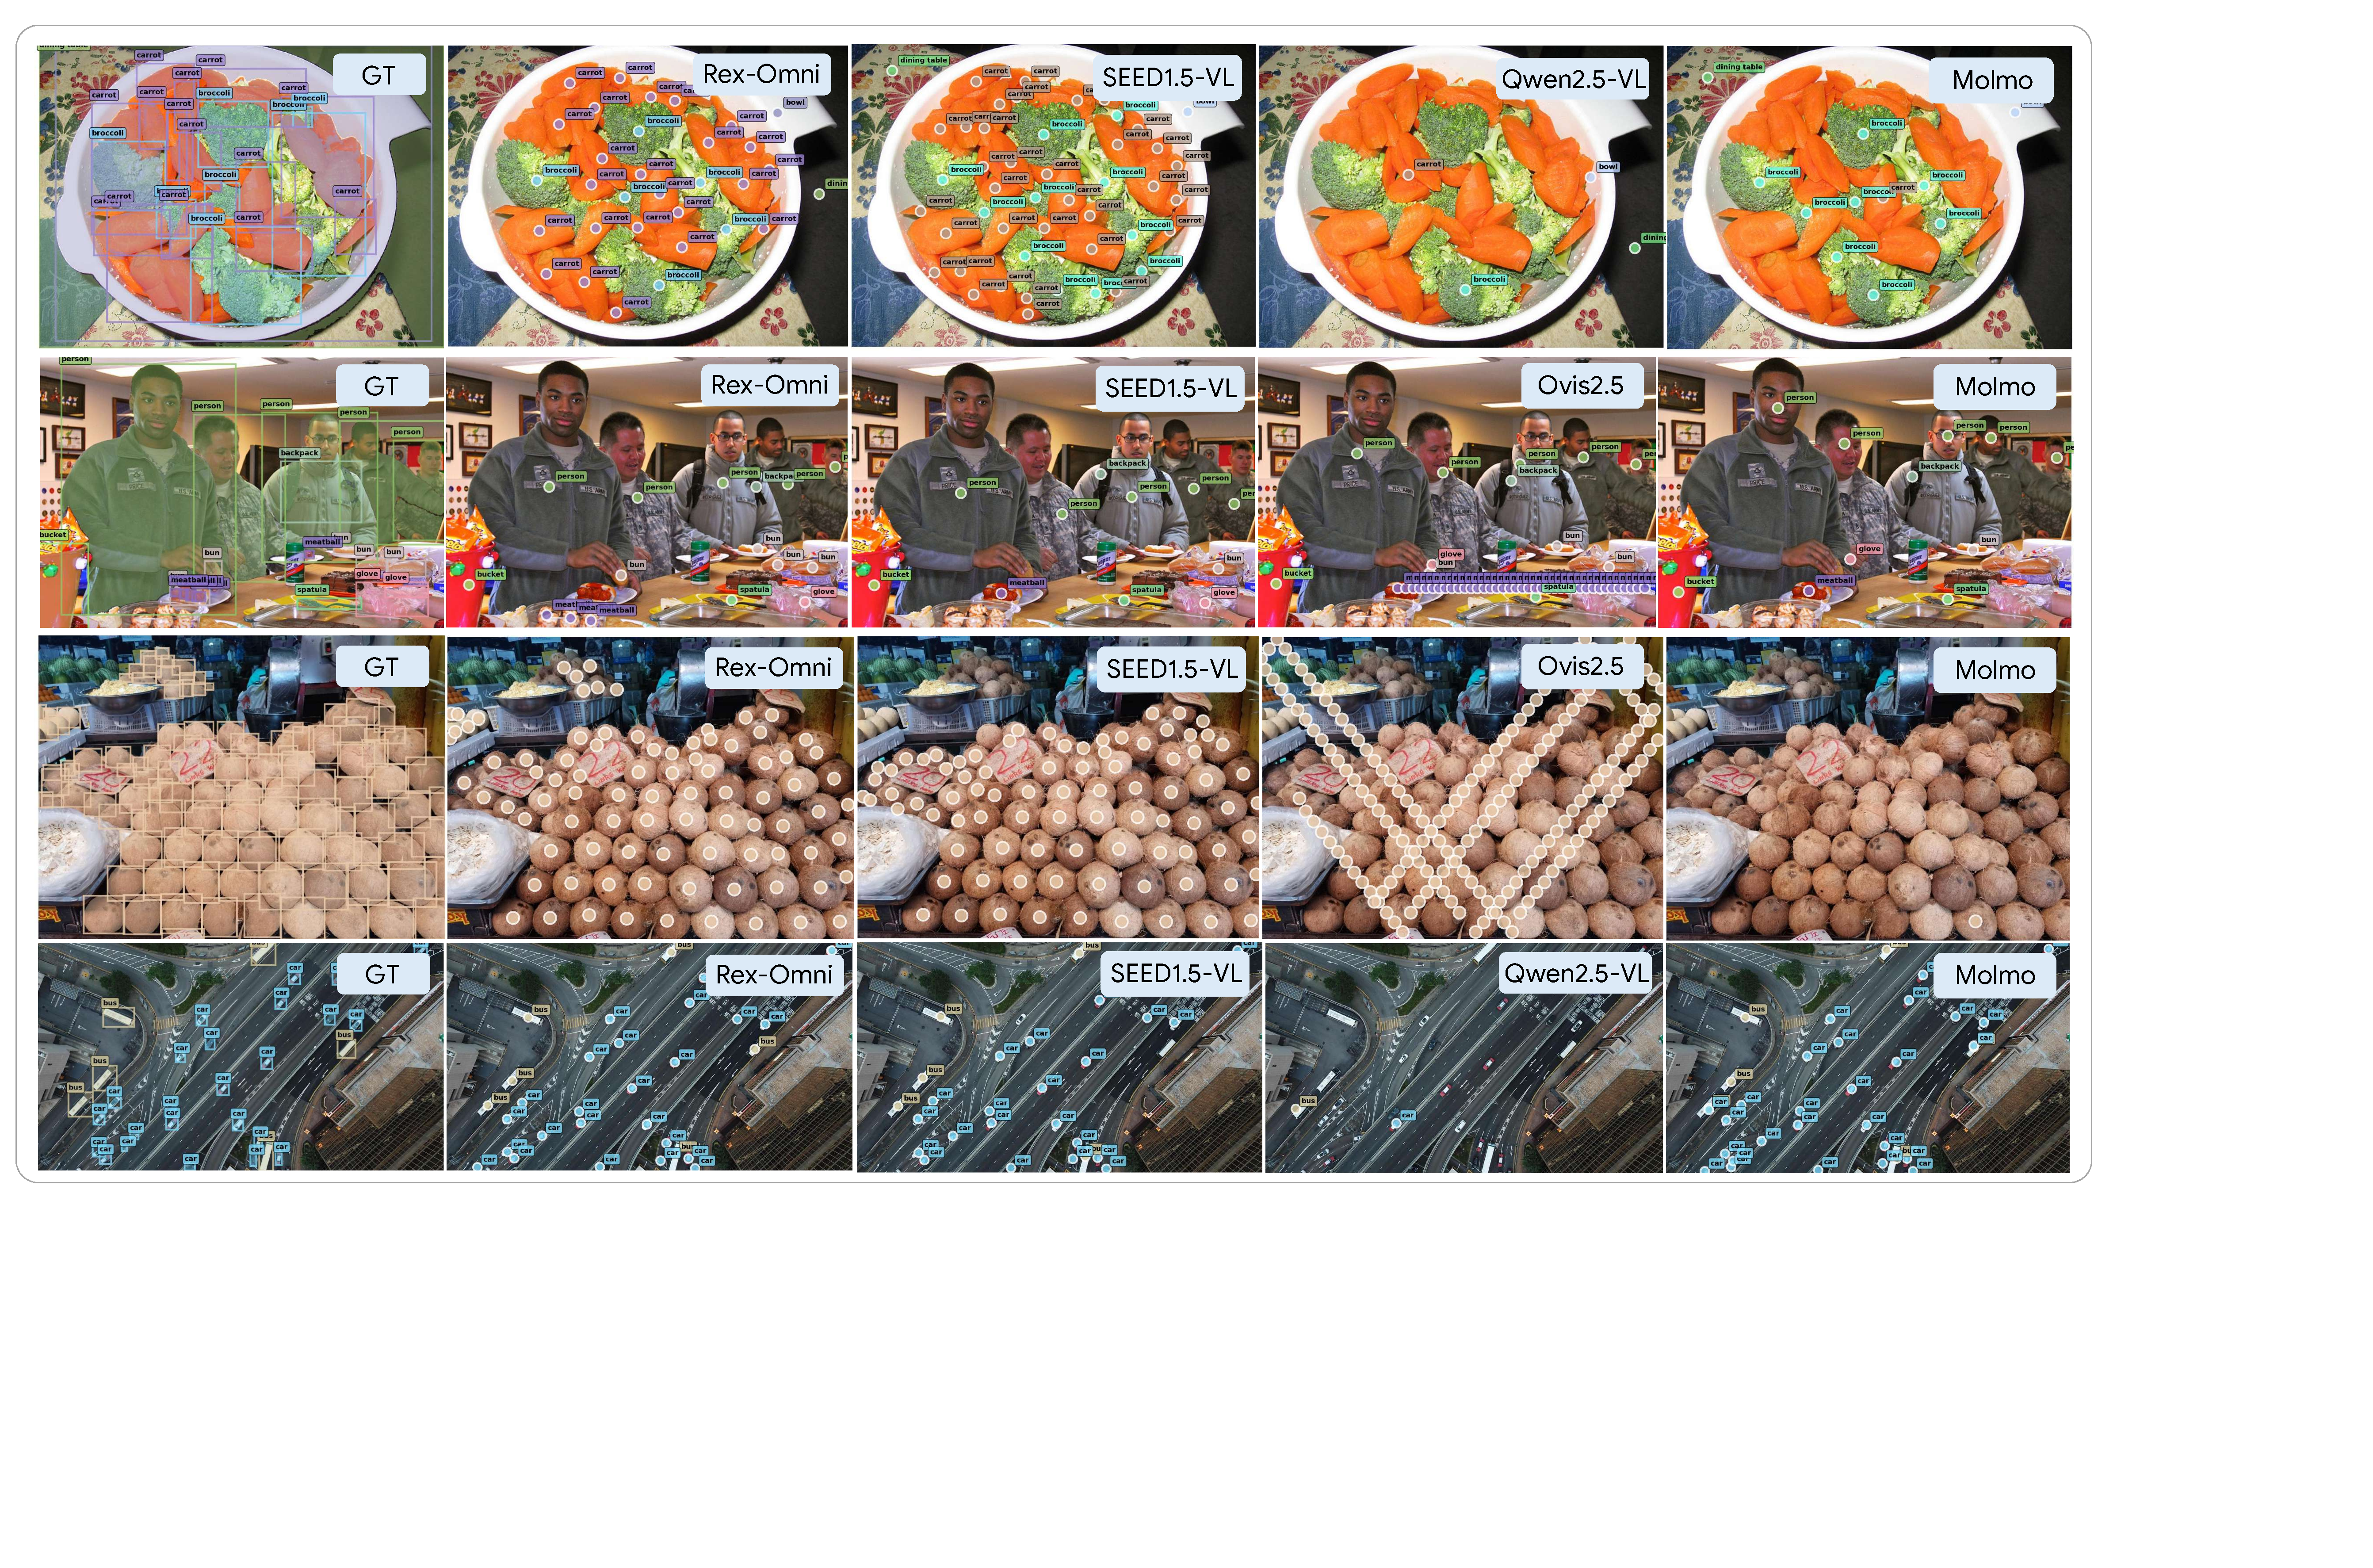
\includegraphics[width=\textwidth]{figures/compare_pointing.pdf}
    \captionsetup{justification=centering}
    \caption{Qualitative comparison of object pointing predictions from different models.}
    \label{fig:compare_pointing}
\end{figure}

\begin{table*}[t]
    \centering
    \resizebox{1.0\textwidth}{!}{
       \begin{tabular}{c|ccccccc|ccccccccccccc}
\toprule
\multirow{3}{*}{Method} & \multicolumn{7}{c|}{ScreenSpot-V2}                                                                                   & \multicolumn{13}{c}{ScreenSpot-Pro}                                                                                                                                                                           \\ \cline{2-21} 
                        & \multicolumn{2}{c}{Mobile}    & \multicolumn{2}{c}{Desktop}   & \multicolumn{2}{c}{Web}       & \multirow{2}{*}{Avg} & \multicolumn{2}{c}{Dev.}      & \multicolumn{2}{c}{Creative}  & \multicolumn{2}{c}{CAD}       & \multicolumn{2}{c}{Sci.}      & \multicolumn{2}{c}{Office}    & \multicolumn{2}{c}{OS}        & Avg           \\ \cline{2-7} \cline{9-21} 
                        & Text          & Icon          & Text          & Icon          & Text          & Icon          &                      & Text          & Icon          & Text          & Icon          & Text          & Icon          & Text          & Icon          & Text          & Icon          & Text          & Icon          &               \\ \midrule
UI-TARS-2B              & 95.2          & 79.1          & 90.7          & 68.6          & 87.2          & 78.3          & 84.7                 & 47.4          & 4.1           & 42.9          & 6.3           & 17.8          & 4.7           & 56.9          & 17.3          & 50.3          & 17.0          & 21.5          & 5.6           & 27.7          \\
Qwen2.5-VL-3B           & 93.4          & 73.5          & 88.1          & 58.6          & {\underline{88.0}}    & 71.4          & 80.9                 & 38.3          & 3.4           & 40.9          & 4.9           & 22.3          & 6.3           & 44.4          & 10.0          & 48.0          & 17.0          & 33.6          & 4.5           & 25.9          \\
UI-R1-3B                & 84.3          & \textbf{96.2} & 75.4          & \textbf{89.2} & 63.6          & \textbf{92.3} & 85.4                 & 22.7          & 4.1           & 27.3          & 3.5           & 11.2          & 6.3           & 42.4          & 11.8          & 32.2          & 11.3          & 13.1          & 4.5           & 17.8          \\
InfiGUI-R1-3B           & -             & -             & -             & -             & -             & -             & -                    & 51.3          & {\underline{12.4}}    & 44.9          & 7.0           & 33.0          & \textbf{14.1} & 58.3          & {\underline{20.0}}    & \textbf{65.5} & 28.3          & \textbf{43.9} & {\underline{12.4}}    & 35.7          \\
SE-GUI-3B               & -             & -             & -             & -             & -             & -             & -                    & 55.8          & 7.6           & 47.0          & 4.9           & \textbf{38.1} & {\underline{12.5}}    & \textbf{61.8} & 16.4          & 59.9          & 24.5          & 40.2          & {\underline{12.4}}    & 35.9          \\
JEDI-3B                 & \textbf{96.6} & 81.5          & {\underline{96.9}}    & 78.6          & \textbf{88.5} & {\underline{83.7}}    & \textbf{88.6}        & 61.0          & \textbf{13.8} & \textbf{53.5} & 8.4           & {\underline{27.4}}    & 9.4           & 54.2          & 18.2          & {\underline{64.4}}    & \textbf{32.1} & {\underline{38.3}}    & 9.0           & {\underline{36.1}}    \\
\rowcolor{lightblue!10} Rex-Omni-SFT            & {\underline{95.5}}    & 80.6          & \textbf{97.4} & 77.1          & 85.5          & 76.4          & 86.4                 & 54.6          & 10.3          & 46.5          & {\underline{10.5}}    & 22.3          & 7.8           & 55.6          & 19.1          & 55.9          & 20.8          & 37.4          & 11.2          & 32.6          \\
\rowcolor{lightblue!10}Rex-Omin-GRPO           & 93.3          & {\underline{84.3}}    & 96.4          & {\underline{84.3}}    & 86.8          & 80.5          & {\underline{88.4}}           & \textbf{61.7} & 9.7           & {\underline{52.5}}    & \textbf{12.6} & 22.3          & 9.4           & {\underline{59.0}}    & \textbf{26.4} & 63.3          & {\underline{28.3}}    & 24.1          & \textbf{15.7} & \textbf{36.8} \\ \bottomrule
\end{tabular}
    }
    \captionsetup{justification=centering}
    \caption{Evaluation results for GUI Grounding task on the ScreenSpot-V2 and ScreenSpot Pro datasets.}
    \label{tab:gui_grounidng}
\end{table*}


\subsection{GUI Grounding}
Graphical User Interface (GUI) grounding evaluates a model’s ability to localize specific UI elements based on natural language queries. This task is critical for applications such as intelligent agents, automated UI interaction, and software testing, as it requires seamless integration of visual perception and language understanding.

\textbf{Benchmarks, Evaluation Setting and Metric: }We evaluate models on two datasets: ScreenSpot-V2~\cite{wu2024atlas} and ScreenSpot-Pro~\cite{li2025screenspot}. ScreenSpot-V2 encompasses mobile, desktop, and web scenarios, featuring a diverse array of UI layouts across 1,272 images. ScreenSpot-Pro, conversely, focuses on ultra-high-resolution interfaces, specifically designed to test the model’s precision in localizing UI elements under highly challenging visual conditions, comprising 1,581 images. Rex-Omni is assessed using its point-based prediction capability, outputting a point within the target UI element for each query. Following standard protocols, we report accuracy, considering a prediction correct if the point falls within the ground-truth bounding box.

\textbf{Results: }As shown in Table \ref{tab:gui_grounidng}, Rex-Omni consistently demonstrates strong performance on GUI grounding tasks. Specifically, among 3B-parameter models, Rex-Omni achieves the highest accuracy across both ScreenSpot V2 and ScreenSpot Pro. This underscores its superior capability to seamlessly integrate robust language understanding with fine-grained visual localization, even in diverse and ultra-high-resolution UI scenarios.


\subsection{Layout Grounding}
Layout grounding requires models to localize and interpret the spatial relationships among elements in a document, such as titles, paragraphs, sections, and figures. This task is crucial for applications like document layout analysis and web page understanding, as it demands not only object detection but also reasoning over structural arrangement and semantic relationships.

\textbf{Benchmark, Evaluation Setting, and Metrics:}
We evaluate our model on the DocLayNet~\cite{pfitzmann2022doclaynet} and M6Doc~\cite{cheng2023m6doc} datasets. DocLayNet is collected from PDF documents and includes 11 categories such as footnotes, pictures, tables, and titles, with a test set consisting of 6,480 images.The M6Doc dataset is considerably more complex, encompassing data from diverse domains (e.g., scientific articles, textbooks, test papers, magazines, newspapers, notes, books) with a total of 74 categories across 2,724 test images. For evaluation, we treat this task as an object detection problem, following the same evaluation protocol used for common object detection on COCO.

\textbf{Results:}
The results are presented in Table~\ref{tab:layout_grounding}. Rex-Omni outperforms other MLLMs by a large margin on layout grounding. While there remains a performance gap compared to closed-set models, Rex-Omni’s ability to handle open-set layout grounding provides a unique advantage. Unlike closed-set models, which are limited to predefined categories, Rex-Omni demonstrates a unique capability to generalize to unseen domains and novel layout structures, establishing it as a more versatile and adaptable solution for real-world layout understanding tasks. Representative visualization results are provided in Figure \ref{fig:compare_layout_grounding} and Figure~\ref{fig:app_layout}.

\begin{table*}[t]
    \centering
    \resizebox{0.9\textwidth}{!}{
        \begin{tabular}{cc|c|ccc|ccc}
\midrule
\multirow{2}{*}{Type} & \multirow{2}{*}{Method} & \multirow{2}{*}{\begin{tabular}[c]{@{}c@{}}Score \\ Thresh.\end{tabular}} & \multicolumn{3}{c|}{DocLayNet} & \multicolumn{3}{c}{M6Doc} \\ \cline{4-9} 
 &  &  & \begin{tabular}[c]{@{}c@{}}F1@IoU\\ 0.5\end{tabular} & \begin{tabular}[c]{@{}c@{}}F1@IoU\\ 0.95\end{tabular} & \begin{tabular}[c]{@{}c@{}}F1@IoU\\ mIoU\end{tabular} & \begin{tabular}[c]{@{}c@{}}F1@IoU\\ 0.5\end{tabular} & \begin{tabular}[c]{@{}c@{}}F1@IoU\\ 0.95\end{tabular} & \begin{tabular}[c]{@{}c@{}}F1@IoU\\ mIoU\end{tabular} \\ \midrule
Closed-Set & DocLayout-YOLO~\cite{zhao2024doclayout} & 0.3 & \textbf{91.2} & \textbf{52.1} & \textbf{81.1} & - & - & - \\ \midrule
\multirow{4}{*}{MLLM}  & Qwen2.5-VL-3B & - & 17.5 & 2.9 & 9.1 & 13.3 & 2.5 & 8.4 \\
 & Qwen2.5-VL-7B & - & 25.6 & 5.1 & 13.4 & 24.0 & 4.1 & 15.0 \\
 & SEED1.5-VL & - & 54.9 & 4.3 & 28.7 & 48.0 & 3.4 & 28.0 \\
 \rowcolor{lightblue!10} & Rex-Omni-SFT & - & 85.9 & 27.2 & 70.7 & {\underline{74.5}} & {\underline{16.2}} & {\underline{54.2}} \\
 \rowcolor{lightblue!10} & Rex-Omni &  & {\underline{89.5}} & {\underline{28.4}} & {\underline{70.7}} & \textbf{76.3} & \textbf{18.7} & \textbf{55.6} \\ \midrule
\end{tabular}
    }
    \centering
    \caption{Performance comparison of different models on the DocLayNet and M6Doc datasets for layout grounding. F1-scores (at IoU=0.5, IoU=0.95, mIoU) are reported.}
    \label{tab:layout_grounding}
\end{table*}

\begin{figure}[t]     
    \centering
    % \hspace*{-0.05\textwidth}
    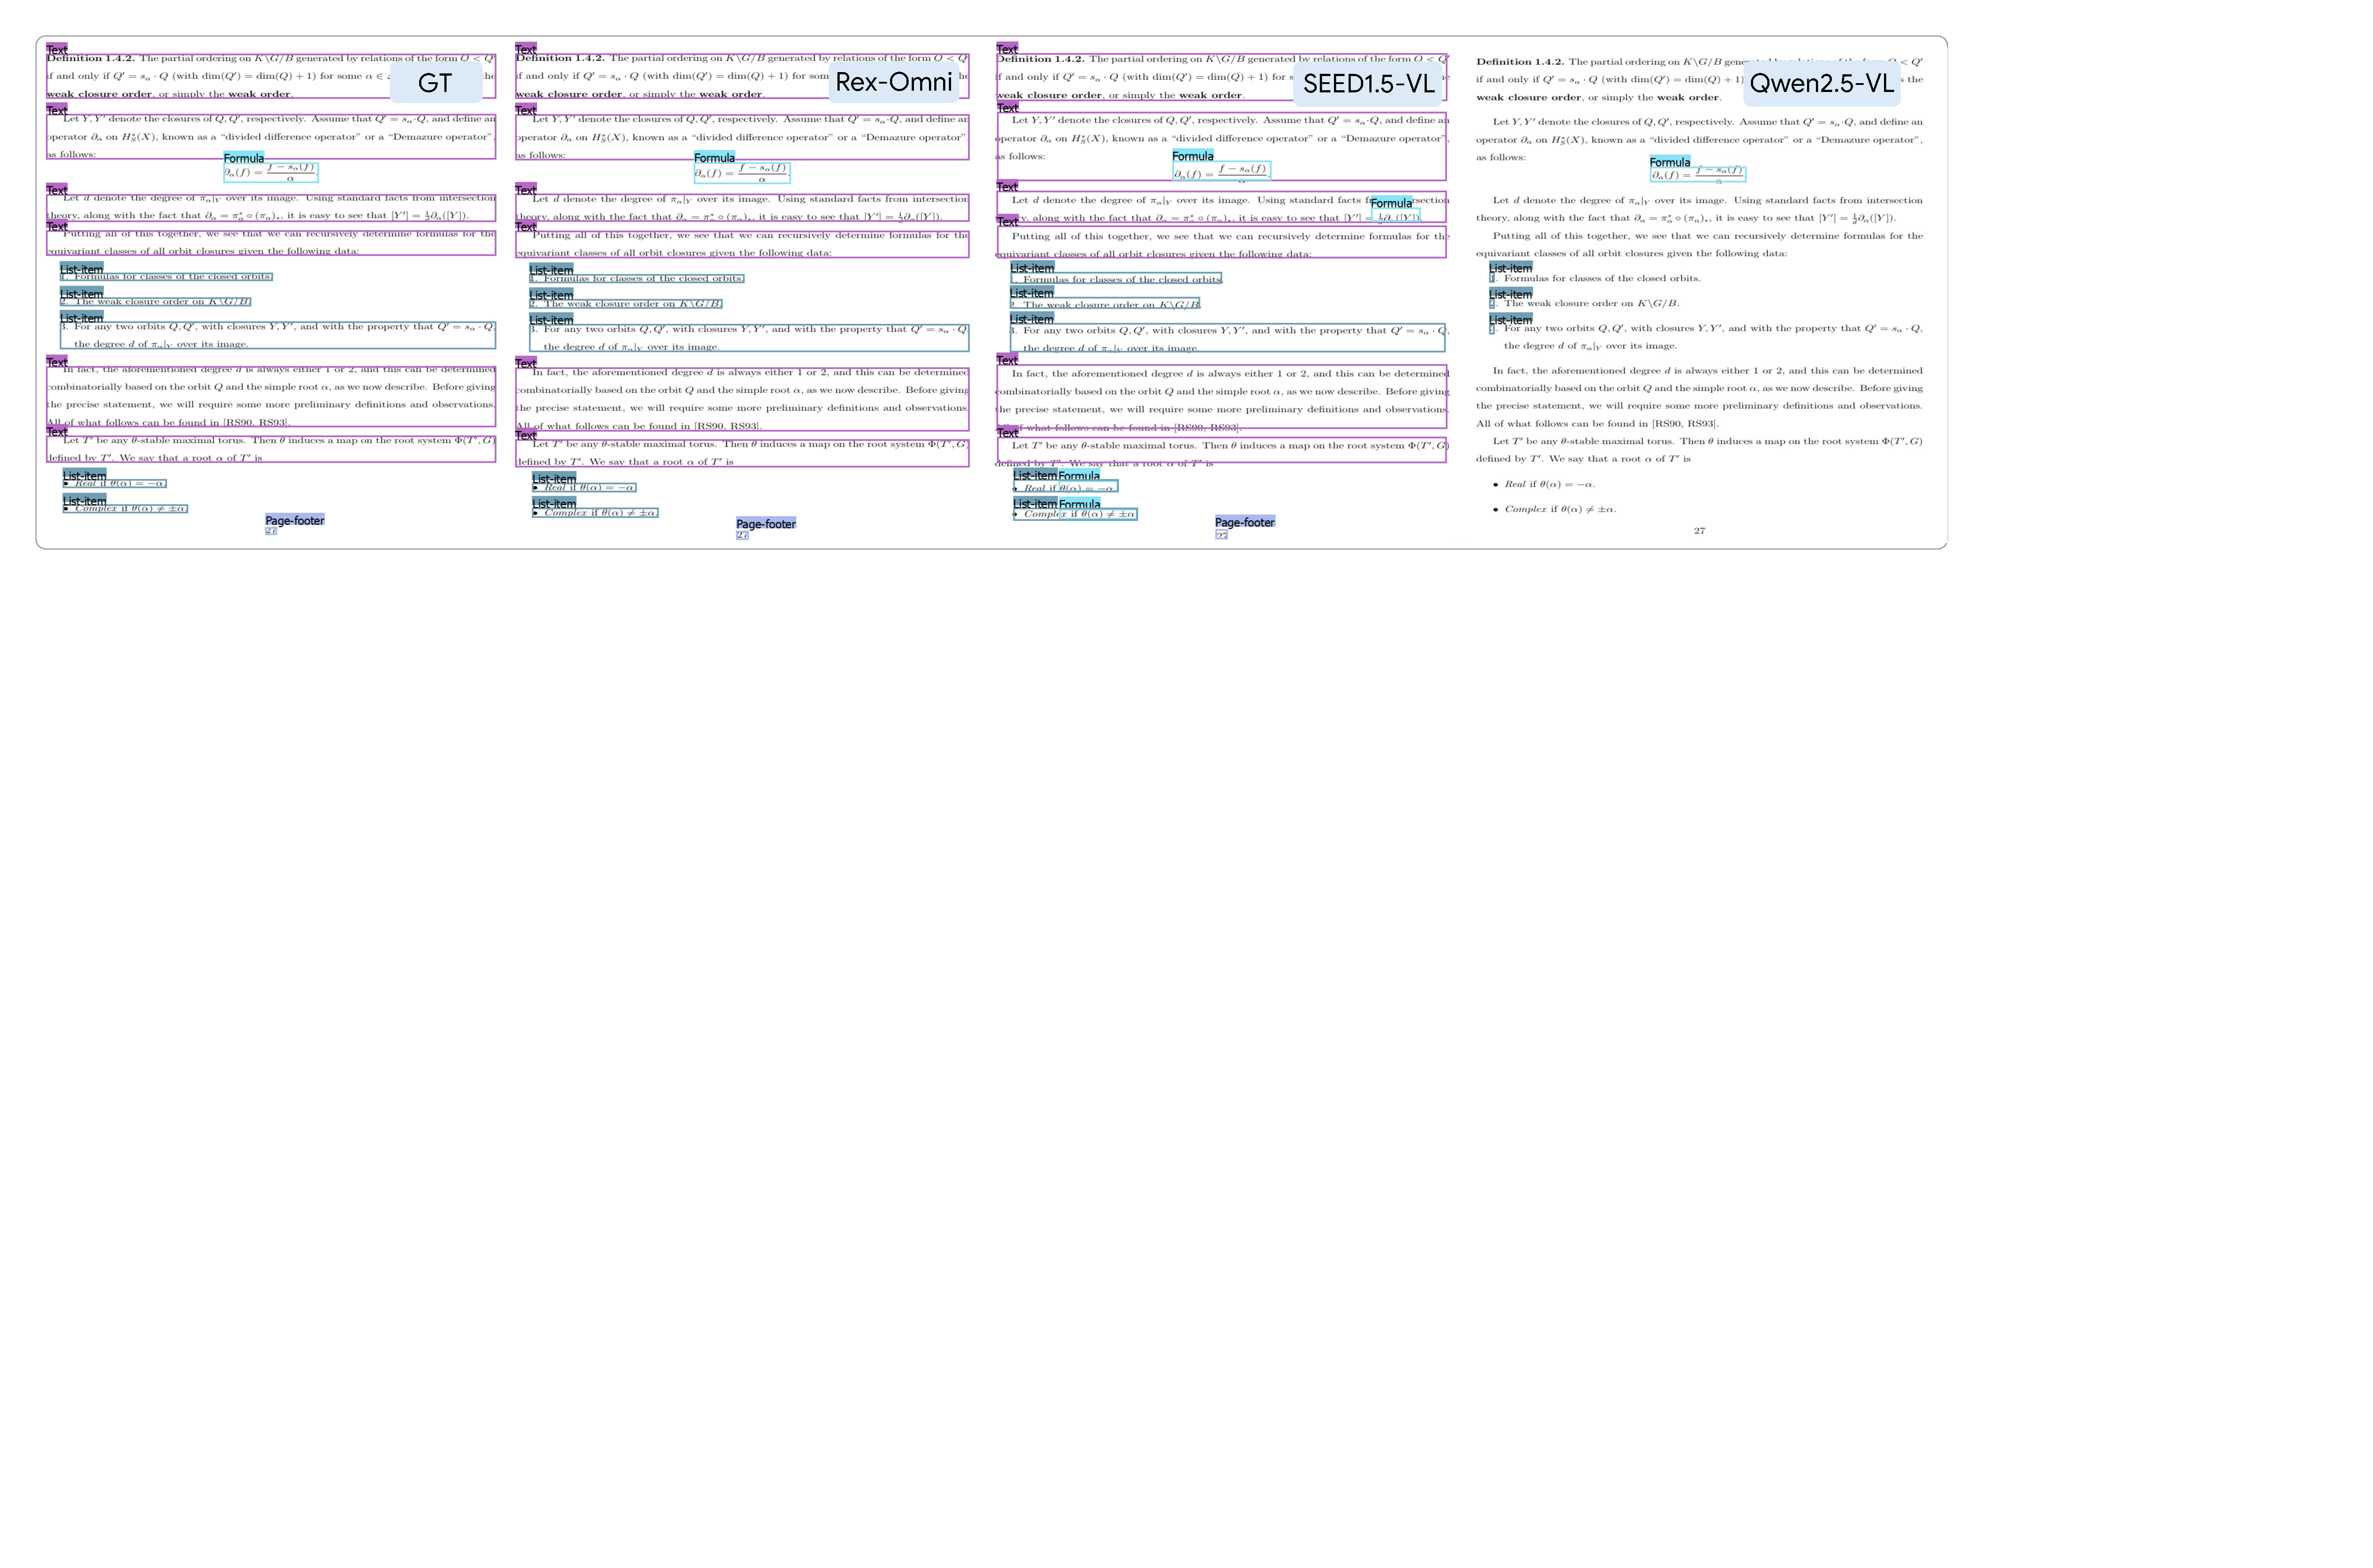
\includegraphics[width=\textwidth]{figures/compare_layout_grounding.pdf}
    \caption{Qualitative comparison of layout grounding predictions from different models. The figure illustrates the models' ability to localize and interpret various layout elements.}
    \label{fig:compare_layout_grounding}
\end{figure}

\begin{table*}[t]
    \centering
    \resizebox{1.0\textwidth}{!}{
        \begin{tabular}{cc|ccc|ccc|ccc|ccc}
\toprule
\multirow{2}{*}{\begin{tabular}[c]{@{}c@{}}Output\\ Format\end{tabular}} & \multirow{2}{*}{Method} & \multicolumn{3}{c|}{HierText} & \multicolumn{3}{c|}{ICDAR2015} & \multicolumn{3}{c|}{TotalText} & \multicolumn{3}{c}{SROIE} \\
\cline{3-14}
 &  & \begin{tabular}[c]{@{}c@{}}F1@IoU\\ 0.5\end{tabular} & \begin{tabular}[c]{@{}c@{}}F1@IoU\\ 0.95\end{tabular} & \begin{tabular}[c]{@{}c@{}}F1@IoU\\ mIoU\end{tabular} & \begin{tabular}[c]{@{}c@{}}F1@IoU\\ 0.5\end{tabular} & \begin{tabular}[c]{@{}c@{}}F1@IoU\\ 0.95\end{tabular} & \begin{tabular}[c]{@{}c@{}}F1@IoU\\ mIoU\end{tabular} & \begin{tabular}[c]{@{}c@{}}F1@IoU\\ 0.5\end{tabular} & \begin{tabular}[c]{@{}c@{}}F1@IoU\\ 0.95\end{tabular} & \begin{tabular}[c]{@{}c@{}}F1@IoU\\ mIoU\end{tabular} & \begin{tabular}[c]{@{}c@{}}F1@IoU\\ 0.5\end{tabular} & \begin{tabular}[c]{@{}c@{}}F1@IoU\\ 0.95\end{tabular} & \begin{tabular}[c]{@{}c@{}}F1@IoU\\ mIoU\end{tabular} \\
\midrule
\multirow{4}{*}{BBOX}
& PaddleOCRv5~\cite{cui2025paddleocr} & 45.2 & \textbf{3.4} & \textbf{30.5} & 38.2 & \textbf{1.2} & 25.6 & 40.2 & 0.7 & 25.7 & \textbf{77.7} & \textbf{5.6} & \textbf{58.6} \\
& SEED1.5-VL & 27.1 & 0.2 & 12.0 & \underline{38.6} & 0.0 & 18.7 & 35.0 & 0.3 & 19.5 & 51.9 & 0.8 & 28.1 \\

& \cellcolor{lightblue!10}Rex-Omni-SFT & \cellcolor{lightblue!10}23.5 & \cellcolor{lightblue!10}0.5 &\cellcolor{lightblue!10} 13.7 & \cellcolor{lightblue!10}31.4 &\cellcolor{lightblue!10} 0.1 & \cellcolor{lightblue!10}18.7 & \cellcolor{lightblue!10}38.1 & \cellcolor{lightblue!10}\underline{1.5} & \cellcolor{lightblue!10}25.0 & \cellcolor{lightblue!10}46.5 & \cellcolor{lightblue!10}0.9 & \cellcolor{lightblue!10}28.6 \\
& \cellcolor{lightblue!10}Rex-Omni & \cellcolor{lightblue!10}\textbf{45.9} & \cellcolor{lightblue!10}1.4 & \cellcolor{lightblue!10}28.0 & \cellcolor{lightblue!10}\textbf{45.2} & \cellcolor{lightblue!10}0.3 & \cellcolor{lightblue!10}\textbf{28.1} & \cellcolor{lightblue!10}\textbf{56.6} & \cellcolor{lightblue!10}\textbf{3.9} & \cellcolor{lightblue!10}\textbf{40.6} & \cellcolor{lightblue!10}72.0 & \cellcolor{lightblue!10}\underline{1.5} & \cellcolor{lightblue!10}44.8 \\
\midrule
\multirow{3}{*}{POLY}
& PaddleOCRv5 & 41.5 & \underline{1.1} & \textbf{26.3} & 36.4 & 0.2 & 23.3 & 34.1 & 0.0 & 18.4 & 70.5 & \textbf{2.3} & \textbf{50.2} \\
& \cellcolor{lightblue!10}Rex-Omni-SFT &\cellcolor{lightblue!10} \textbf{43.2} & \cellcolor{lightblue!10}\underline{0.3} &\cellcolor{lightblue!10} 26.2 & \cellcolor{lightblue!10}43.2 & \cellcolor{lightblue!10}\textbf{0.3} & \cellcolor{lightblue!10}26.2 & \cellcolor{lightblue!10}50.3 & \cellcolor{lightblue!10}0.1 & \cellcolor{lightblue!10}\textbf{25.7} & \cellcolor{lightblue!10}\textbf{73.8} & \cellcolor{lightblue!10}0.2 & \cellcolor{lightblue!10}39.7 \\
& \cellcolor{lightblue!10}Rex-Omni &\cellcolor{lightblue!10} 40.2 & \cellcolor{lightblue!10}0.1 & \cellcolor{lightblue!10}20.2 & \cellcolor{lightblue!10}\textbf{50.7} & \cellcolor{lightblue!10}0.0 & \cellcolor{lightblue!10}\textbf{28.5} & \cellcolor{lightblue!10}\textbf{52.8} & \cellcolor{lightblue!10}\textbf{0.1} & \cellcolor{lightblue!10}25.6 & \cellcolor{lightblue!10}60.3 & \cellcolor{lightblue!10}0.0 & \cellcolor{lightblue!10}19.2 \\
\bottomrule
\end{tabular}
    }
    \caption{Performance comparison of various models on the OCR task, evaluated using F1 score for text detection and recognition accuracy.}
    \label{tab:ocr}
\end{table*}


\begin{figure}[t]     
    \centering
    % \hspace*{-0.05\textwidth}
    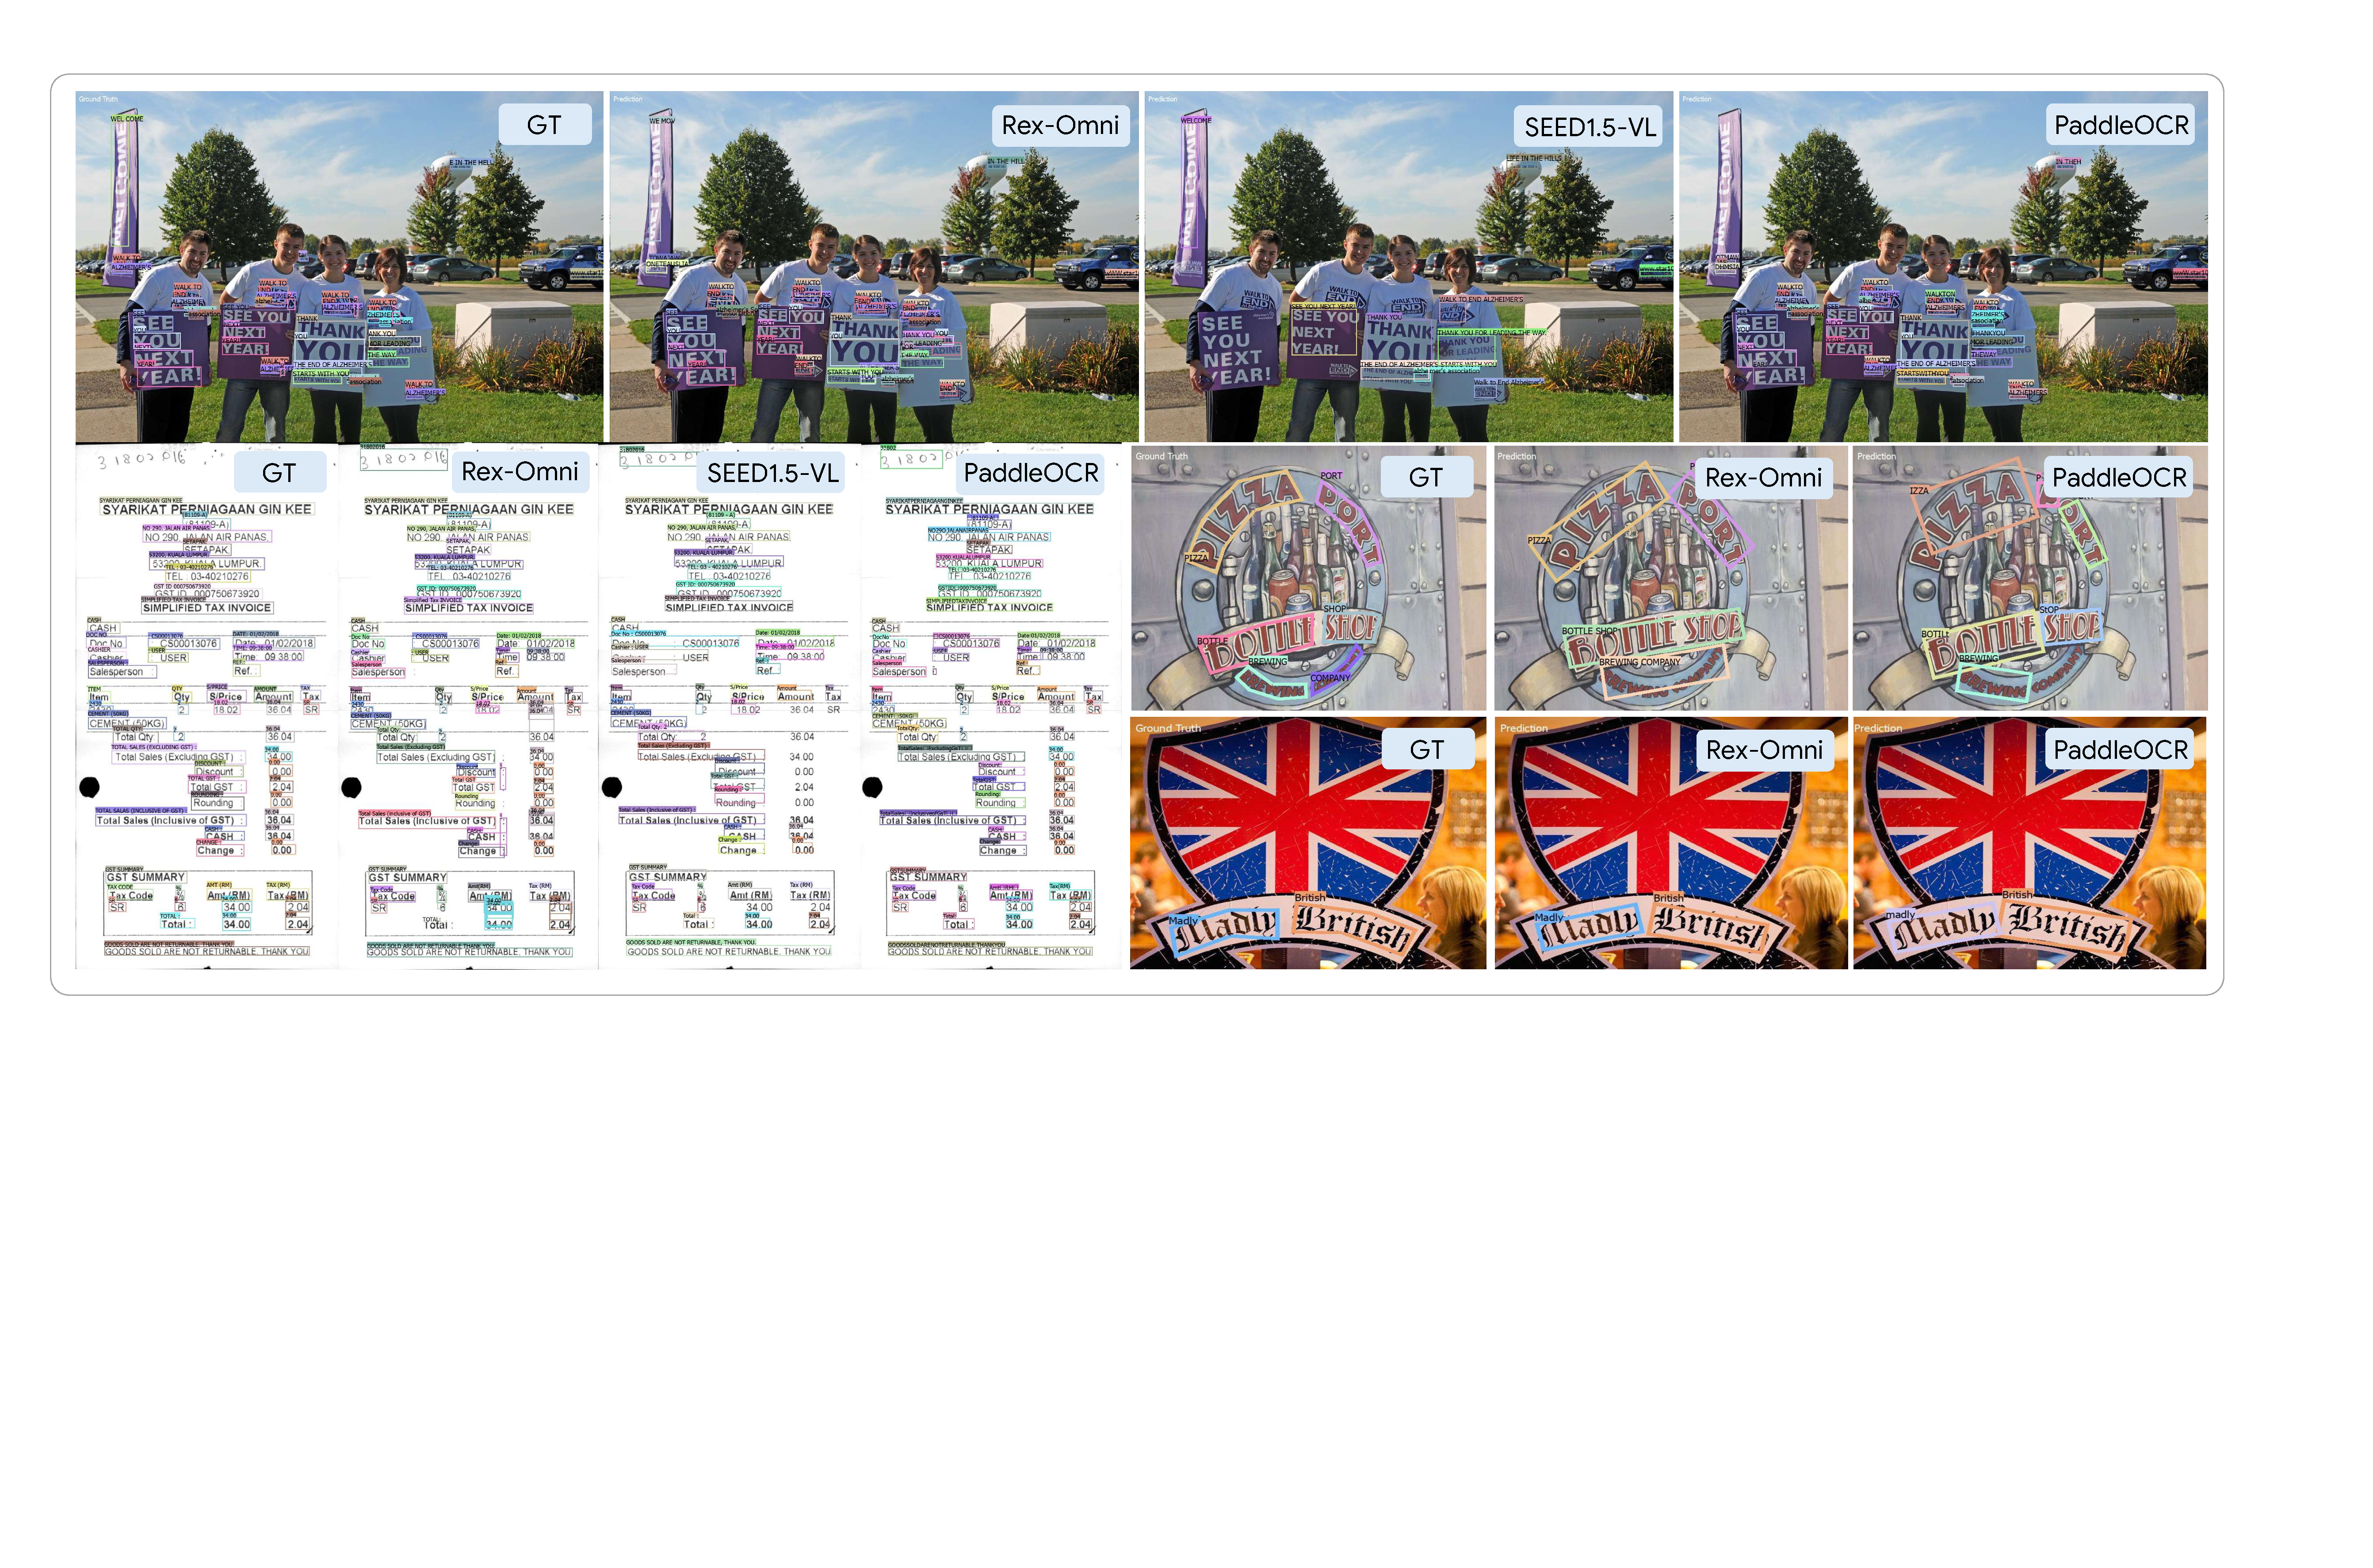
\includegraphics[width=\textwidth]{figures/compare_ocr.pdf}
    \captionsetup{justification=centering}
    \caption{Visualization of OCR results across models.}
    \label{fig:compare_ocr}
\end{figure}

\subsection{OCR}
Optical Character Recognition (OCR) involves both text detection and recognition, where the model identifies and extracts text from images or documents. The task requires the model to detect text regions and then recognize the characters or words within those regions, enabling the conversion of scanned documents or images into machine-readable text.

\textbf{Benchmark, Evaluation Setting:}
We evaluate the performance of PaddleOCR, SEED1.5-VL, and Rex-Omni on four diverse datasets. The core evaluation method involves detecting and recognizing all text within the images. The datasets include HierText (3,446 instances, primarily dense text), TotalText (600 instances, scene text with predominantly curved text), ICDAR2015 (1,000 instances, scene text), and SROIE (720 instances, printed receipt data with mostly horizontal text). Together, these datasets cover a broad spectrum of OCR challenges, from dense and curved scene text to structured document text. For PaddleOCR and Rex-Omni, both bounding box (BBOX) and polygonal (POLY) text regions are predicted, and we report performance for both formats to provide a comprehensive assessment of text localization.

\textbf{Metrics:} We formulate OCR as an object detection task, following the COCO evaluation protocol with categories replaced by recognized text. A prediction is considered correct if (1) the predicted and ground-truth regions match, and (2) the recognized text exactly matches the ground truth. Performance is reported using the F1 score, balancing precision and recall.

\textbf{Results:} The evaluation results for the OCR task are presented in Table \ref{tab:ocr}. For bounding box (BBOX) outputs, Rex-Omni demonstrates strong competitive performance. It significantly outperforms SEED1.5-VL across all metrics and datasets, and achieves comparable or superior results to the dedicated OCR expert model PaddleOCRv5 in several key aspects. This highlights Rex-Omni's robust capabilities in text detection and recognition using bounding boxes. In the polygonal (POLY) output format, Rex-Omni also shows competitive performance. The full Rex-Omni model, after GRPO post-training, notably achieves leading results on challenging datasets like ICDAR2015 for polygonal text region detection. This indicates the versatility of our approach in handling more complex text geometries. Consistent gains from Rex-Omni-SFT to Rex-Omni further validate the effectiveness of our two-stage training pipeline in enhancing OCR performance. Representative visualization results are provided in Figure \ref{fig:compare_ocr} and and Figure~\ref{fig:app_ocr}.

\begin{table}[!t]
\centering
\renewcommand{\arraystretch}{1.2}
\resizebox{1.0\textwidth}{!}{
\begin{tabular}{c|c|ccccc|cc}
\toprule
Multi Subtask &
\multicolumn{1}{c|}{\textit{Proprietary Models}} &
\multicolumn{5}{c|}{\textit{Referring Specialist Models}} & \multicolumn{2}{c}{\textit{Our Models}}  \\
% \cline{2-8}
& Gemini-2.5-Pro~\cite{comanici2025gemini} & SpaceLLAVA~\cite{foutter2024space} & RoboPoint~\cite{yuan2024robopoint} & Molmo-7B~\cite{deitke2024molmo} & Molmo-72B~\cite{deitke2024molmo} & ReboRefer-2B$^{*}$~\cite{zhou2025roborefer} & \cellcolor{lightblue!10} Rex-Omini-SFT & \cellcolor{lightblue!10} Rex-Omini \\
\hline
\textit{Location} & 46.96 & 5.82 & 22.87 & 21.91 & 45.77 & 51.00 &  \cellcolor{lightblue!10} \textbf{55.00} & \cellcolor{lightblue!10} \underline{54.00} \\
\textit{Placement} & 24.21 & 4.31 & 9.27  & 12.85 & 14.74 & \underline{49.00} & \cellcolor{lightblue!10} 45.00 & \cellcolor{lightblue!10} \textbf{50.00} \\
\textit{Useen} & 27.14 & 4.02 & 8.40  & 12.23 & 21.24 & \textbf{38.96} & \cellcolor{lightblue!10}\underline{36.36} & \cellcolor{lightblue!10}\underline{36.36}  \\
\bottomrule
\end{tabular}
}
\caption{Comparison of different models on the RefSpatial benchmark. The value is the percentage (\%) of correct predictions. *: evaluated without depth prior.}
\label{tab:spatial}
\end{table}

\begin{figure}[t]     
    \centering
    % \hspace*{-0.05\textwidth}
    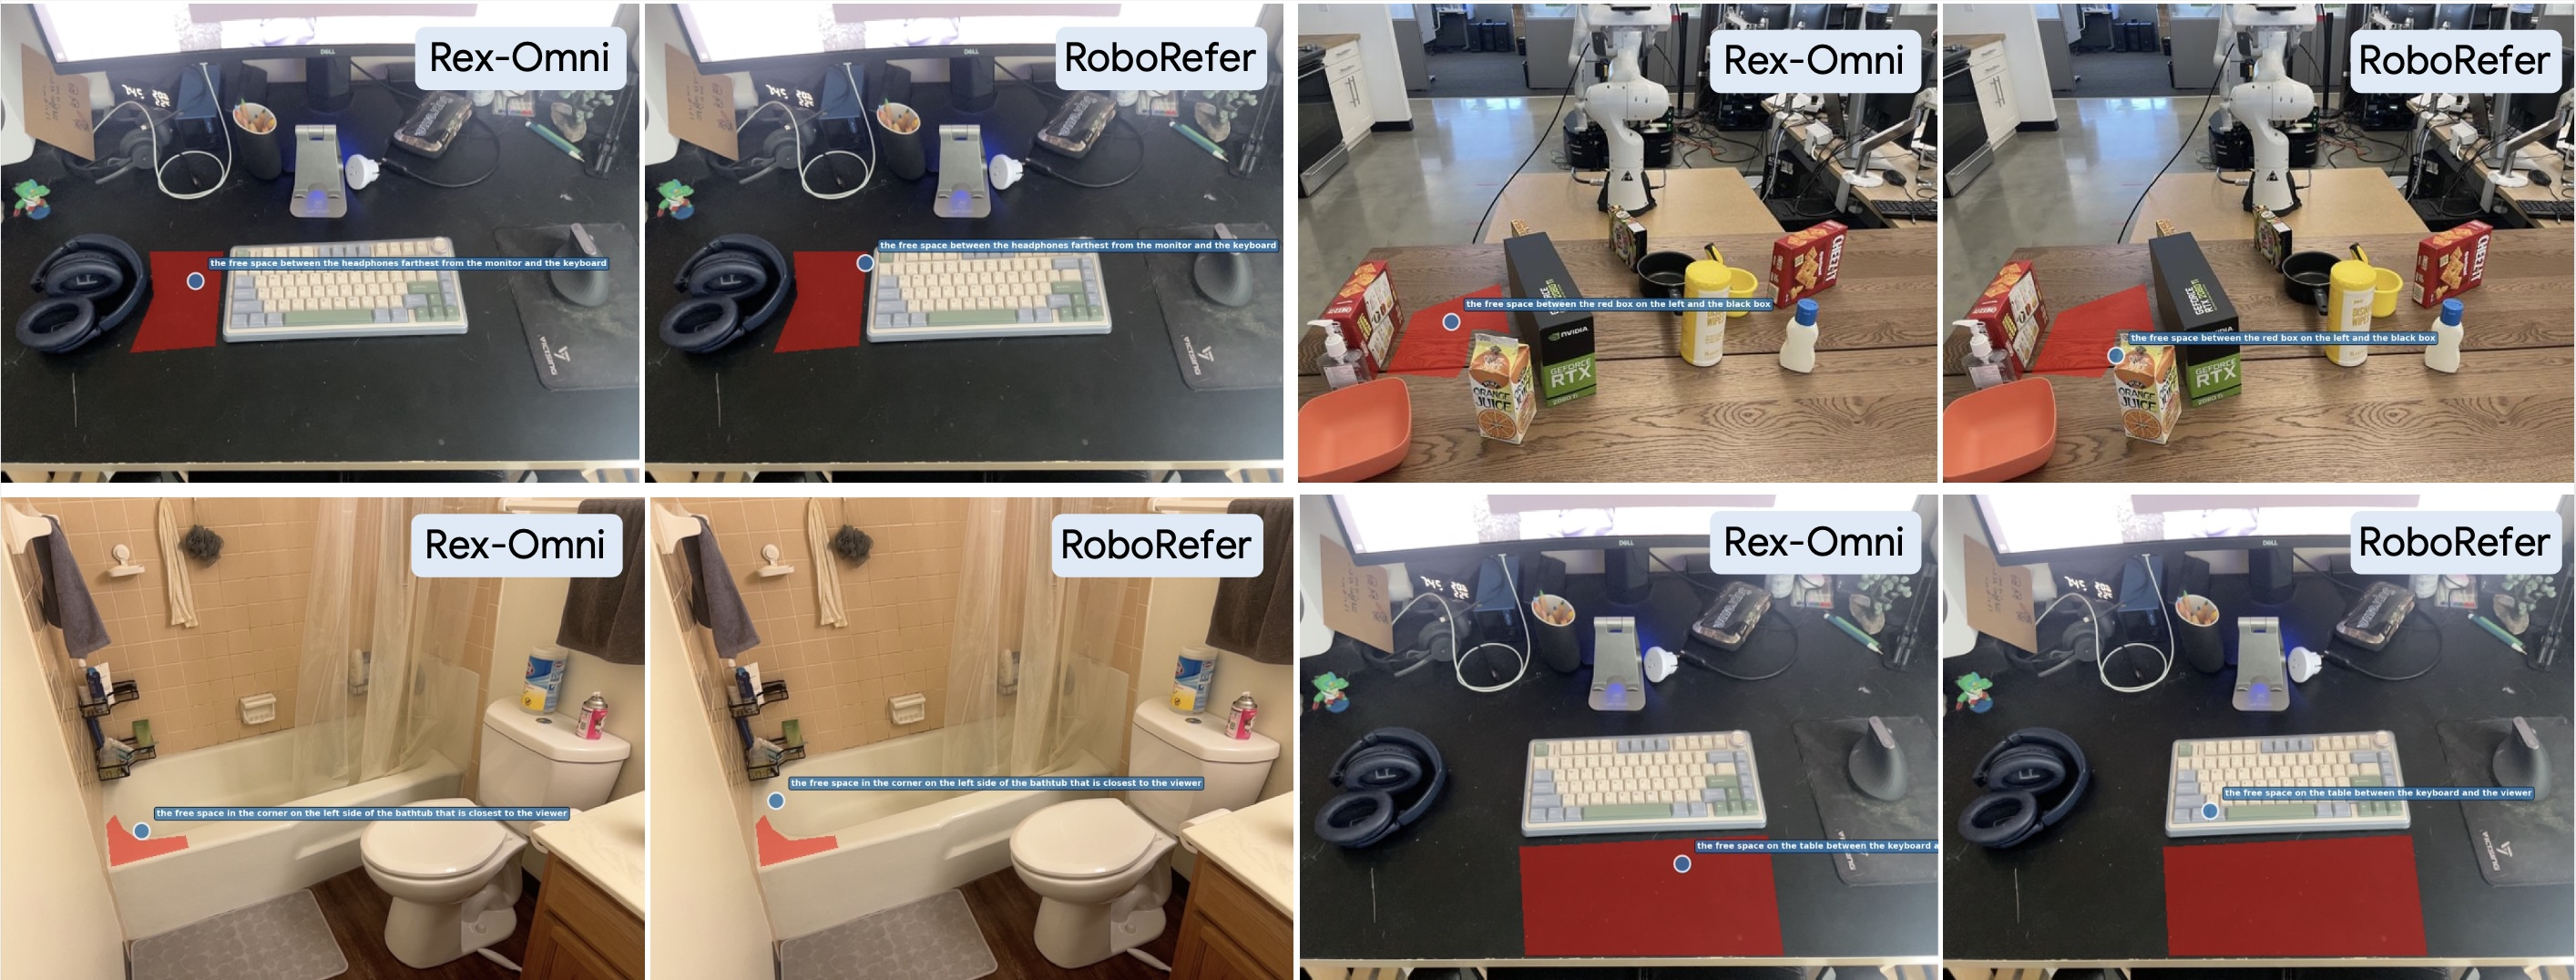
\includegraphics[width=\textwidth]{figures/compare_spatial.jpg}
    \captionsetup{justification=centering}
    \caption{Visualization of Spatial Pointing results across models. Masks indicate correct areas.}
    \label{fig:compare_spatial}
\end{figure}


\subsection{Spatial Pointing}

This task focuses on grounding natural language expressions that describe spatial relationships in complex scenes. Unlike standard referring object detection, which primarily matches objects to category names or simple attributes, spatial grounding requires models to interpret relational cues such as relative position, anchoring, and free-space placement.

\noindent\textbf{Benchmark and Metrics:}
RefSpatial-Bench~\cite{zhou2025roborefer} evaluates spatial referring and reasoning in complex indoor scenes across two tasks: \textit{location} and \textit{placement}, each with 100 curated samples. Each sample includes an image, a natural language referring expression, and precise mask annotations. The location task requires models to predict a 2D point corresponding to a target object based on referring expressions that may involve attributes such as color, shape, spatial order, or anchor-based references. The placement task requires identifying a suitable 2D point within a free space described in the expression, often involving multiple anchors or hierarchical spatial relations. To assess generalization, the benchmark additionally provides 77 unseen samples containing novel combinations of spatial relations not present in training. Evaluation is performed using ground-truth masks, with accuracy defined as the percentage of predictions falling within the mask region.

\noindent\textbf{Results:} As shown in Table~\ref{tab:spatial}, Rex-Omni substantially outperforms prior proprietary and referring-specialist models. Its strong performance on both location and placement tasks suggests enhanced applicability to downstream scenarios such as robotic manipulation, where accurate grasping and placement are essential. Moreover, Rex-Omni demonstrates superior generalization to unseen cases, underscoring its robustness in handling novel spatial relations. Representative visualization results are provided in Figure \ref{fig:compare_spatial}.

\subsection{Keypoint}

\noindent\textbf{Benchmark, Evaluation Setting, and Metrics:}
COCO is a benchmark dataset designed to evaluate 2D human pose estimation and instance-level keypoint detection capabilities in unconstrained environments. It comprises a large-scale collection of images featuring people in diverse and complex natural scenes. Each annotated person instance includes a set of 17 predefined body joints, forming a standard human skeleton. AP10K is a benchmark designed to advance the field of 2D animal pose estimation, addressing the challenge of anatomical variation across species. The benchmark standardizes keypoint annotation with a unified definition of 17 body keypoints for mammals, reptiles, and birds.
Following the COCO protocol, we adopt Object Keypoint Similarity (OKS) as the evaluation metric. We report F1 score at OKS thresholds of 0.5, 0.95, and the mean over thresholds from 0.5 to 0.95 in increments of 0.05.

\begin{table*}[t]
    \centering
    \resizebox{1.0\textwidth}{!}{
       \begin{tabular}{cc|c|ccc|ccc}
\toprule
\multirow{2}{*}{Type} & \multirow{2}{*}{Model} & \begin{tabular}[c]{@{}c@{}}Score\\ Thresh.\end{tabular} 
& \multicolumn{3}{c|}{COCO Keypoint} & \multicolumn{3}{c}{AP10K Keypoint} \\
\cline{4-9}
 &  &  & \begin{tabular}[c]{@{}c@{}}F1@OKS\\ 0.5\end{tabular} & \begin{tabular}[c]{@{}c@{}}F1@OKS\\ 0.95\end{tabular} & \begin{tabular}[c]{@{}c@{}}F1@OKS\\ mOKS\end{tabular} 
 & \begin{tabular}[c]{@{}c@{}}F1@OKS\\ 0.5\end{tabular} & \begin{tabular}[c]{@{}c@{}}F1@OKS\\ 0.95\end{tabular} & \begin{tabular}[c]{@{}c@{}}F1@OKS\\ mOKS\end{tabular} \\
\midrule
Open-set & X-Pose & \begin{tabular}[c]{@{}c@{}}0.3 (COCO) or\\ 0.05 (AP10K)\end{tabular} 
& \textbf{66.3} & \textbf{39.6} & \textbf{57.2} & 17.0 & 2.1 & 8.7 \\
\midrule
\multirow{2}{*}{MLLM} 
& Rex-Omni-SFT & - & 39.9 & 17.5 & 29.3 & 27.4 & 2.2 & 13.0 \\
& Rex-Omni & - & 44.4 & 17.9 & 32.6 & \textbf{30.1} & \textbf{3.0} & \textbf{14.6} \\
\bottomrule
\end{tabular}
    }
    \captionsetup{justification=centering}
    \caption{Evaluation results for keypoint estimation on COCO and AP10K datasets.}
    \label{tab:keypointing}
\end{table*}


\begin{figure}[t]     
    \centering
    % \hspace*{-0.05\textwidth}
    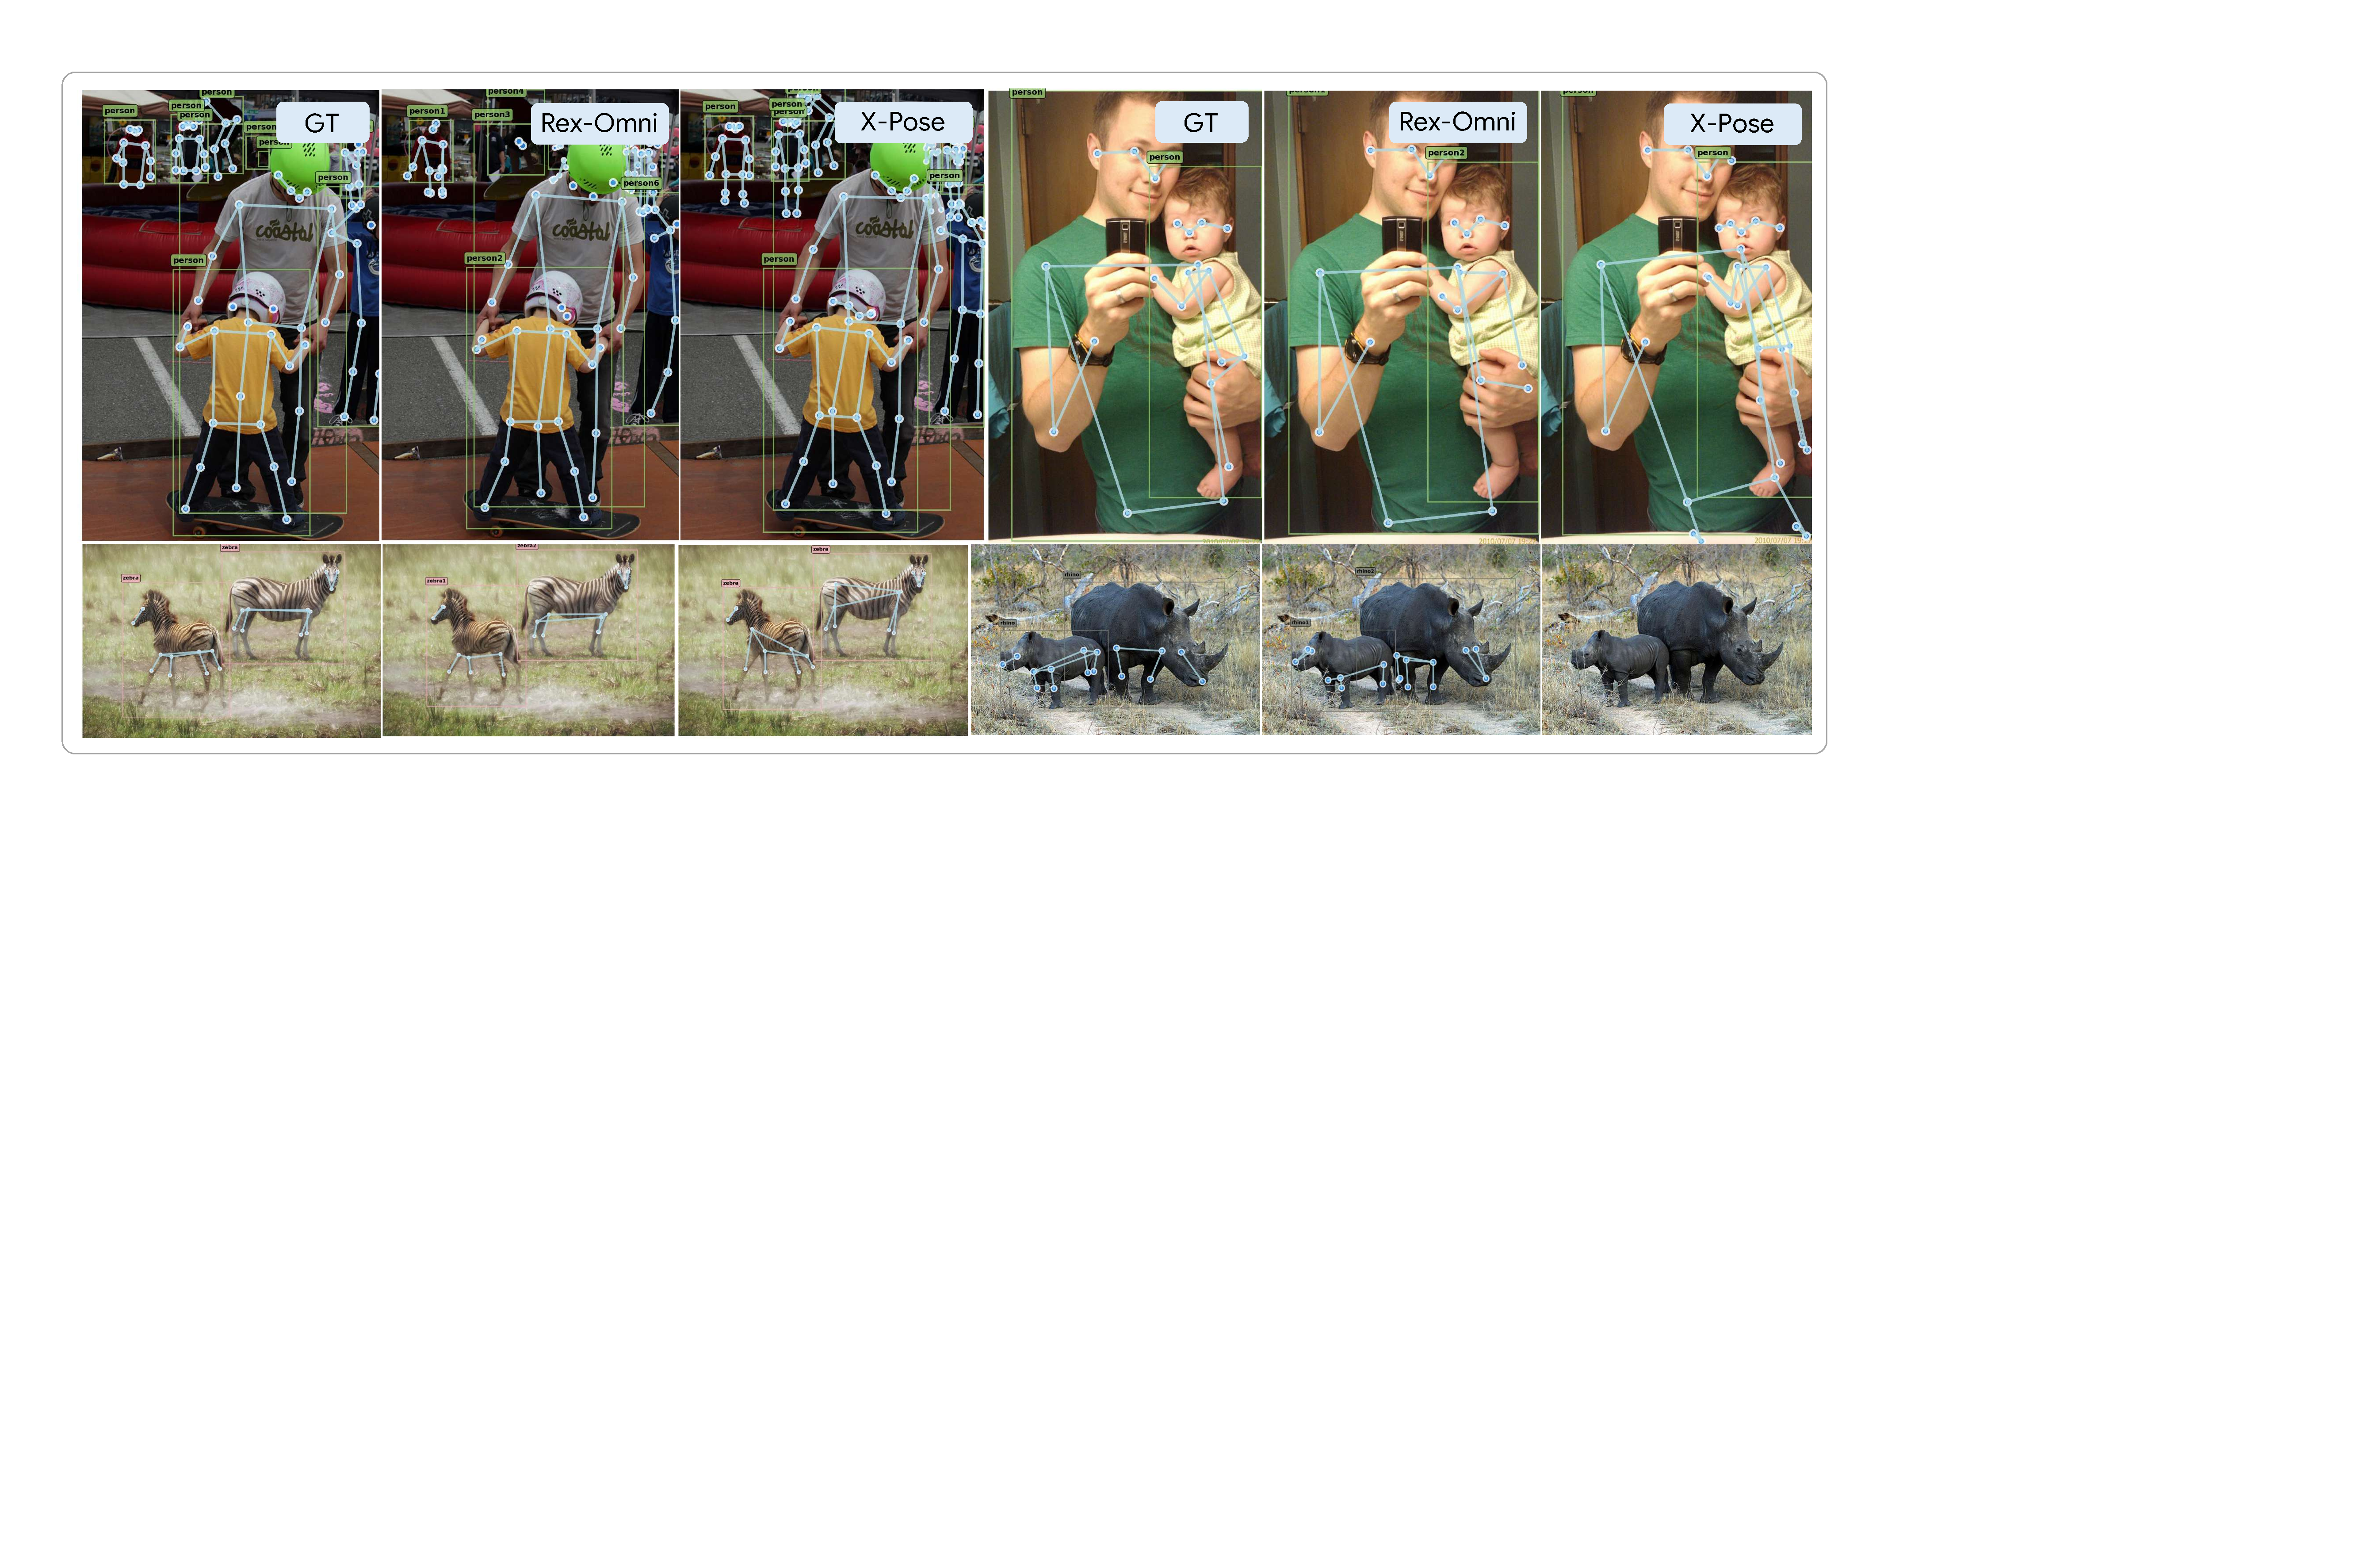
\includegraphics[width=\textwidth]{figures/compare_keypoint.pdf}
    \captionsetup{justification=centering}
    \caption{Qualitative comparison of keypoint detection predictions from different models.}
    \label{fig:keypoint}
\end{figure}


\noindent\textbf{Results:} 
As shown in Table~\ref{tab:keypointing}, the open-set expert model X-Pose achieves the strongest performance on COCO keypoint detection, particularly at lower OKS thresholds. However, it generalizes poorly to AP10K, where its performance drops sharply. In contrast, Rex-Omni demonstrates more balanced results across both human and animal keypoint benchmarks. Although its absolute scores on COCO lag behind X-Pose, Rex-Omni substantially outperforms it on AP10K, highlighting its superior cross-domain generalization. Furthermore, the consistent improvement from Rex-Omni-SFT to the full Rex-Omni model validates the effectiveness of our two-stage training pipeline for enhancing keypoint reasoning. Representative visualization results are provided in Figure \ref{fig:keypoint}.
